% !TeX program = xelatex
\documentclass[10pt, a4paper, oneside]{ctexart}
\usepackage{amsmath, amsthm, amssymb, appendix, bm, fancyhdr}
\usepackage{amsfonts, mathtools, mathrsfs}
\usepackage{diagbox, graphicx, geometry, hyperref, lipsum, longtable, titlesec, textcomp, zhnumber}
\usepackage{booktabs, caption, subcaption, enumitem, float, multirow, array}
\usepackage{xcolor}

\renewcommand{\abstractname}{\Large\textbf{摘要}}
\renewcommand{\thesection}{\zhnum{section}}
\renewcommand{\thesubsection}{\arabic{section}.\arabic{subsection}}
\numberwithin{equation}{section}
\numberwithin{table}{section}
\numberwithin{figure}{section}
\renewcommand{\theequation}{\arabic{section}.\arabic{equation}}
\renewcommand{\thetable}{\arabic{section}.\arabic{table}}
\renewcommand{\thefigure}{\arabic{section}.\arabic{figure}}

\title{\textbf{二维复杂分布的生成建模与评价}\\[0.6em]\large 基于 VAE 与扩散模型的比较研究}
\author{刘世阳\quad PB23050876}
\date{2026 年 6 月}
\linespread{1.5}
\geometry{left=2.9cm, right=2.9cm, top=3.18cm, bottom=3.18cm}
\newtheorem{theorem}{定理 \arabic{section}.\hspace{-5pt}}
\newtheorem{definition}{定义 \arabic{section}.\hspace{-5pt}}
\newtheorem{lemma}{引理 \arabic{section}.\hspace{-5pt}}
\newtheorem{corollary}{推论 \arabic{section}.\hspace{-5pt}}
\newtheorem{example}{例 \arabic{section}.\hspace{-5pt}}
\newtheorem{proposition}{命题 \arabic{section}.\hspace{-5pt}}

\newcommand{\R}{\mathbb{R}}
\newcommand{\Ncal}{\mathcal{N}}
\newcommand{\E}{\mathbb{E}}
\newcommand{\KL}{D_{\mathrm{KL}}}
\newcommand{\norm}[1]{\left\| #1 \right\|}
\newcommand{\vect}[1]{\mathbf{#1}}
\newcommand{\mat}[1]{\boldsymbol{#1}}

\graphicspath{{../figures/analysis/}{../figures/generation/}{../figures/evaluation/}{../figures/extensions/}{../figures/}}
\hypersetup{
    colorlinks=true,
    linkcolor=black,
    citecolor=black,
    urlcolor=blue,
    pdfborder={0 0 0},
}
\setlength{\emergencystretch}{2em}
\setcounter{topnumber}{4}
\setcounter{bottomnumber}{3}
\setcounter{totalnumber}{6}
\renewcommand{\topfraction}{0.92}
\renewcommand{\bottomfraction}{0.82}
\renewcommand{\textfraction}{0.06}
\renewcommand{\floatpagefraction}{0.86}
\setlength{\floatsep}{8pt plus 2pt minus 2pt}
\setlength{\textfloatsep}{10pt plus 2pt minus 3pt}
\setlength{\intextsep}{8pt plus 2pt minus 2pt}
\captionsetup{font=small, labelfont=normalfont, textfont=normalfont, skip=5pt}
\renewcommand{\arraystretch}{1.08}

\begin{document}
\maketitle
\setcounter{page}{0}
\thispagestyle{empty}

% ==================== 摘要 ====================
\begin{abstract}
{\fontsize{10}{15}\selectfont
本文研究 Gaussian Mixture、Ring、Two Moons 和 Spiral 四类二维复杂分布的生成建模问题，比较变分自编码器（VAE）与去噪扩散概率模型（DDPM）在不同几何结构上的表现。本文首先通过局部 $k$ 近邻统计、有效维度和极坐标分析刻画数据的多峰性、流形厚度与拓扑难点；随后建立 VAE 与 DDPM，并用 MMD、Wasserstein 距离、Coverage 和 Precision 评价生成质量。实验显示，默认配置下 DDPM 在连续流形的支撑集保持上整体更稳，而 VAE 具有训练稳定和采样快速的优势。进一步的潜空间诊断表明，VAE 的主要问题并非完全后验崩塌，而是 KL 压缩导致的潜空间低利用和解码插值；适度降低 KL 权重可改善覆盖，但过弱 KL 会破坏先验采样。针对 DDPM 在 Spiral 上仍难恢复双臂结构的问题，本文引入螺旋臂编号、相位和局部残差构成的结构坐标，使曲线外比例由 $0.487$ 降至 $0.048$。结果说明，复杂拓扑分布的生成质量不仅取决于模型容量，也取决于是否显式表达数据的结构变量。
\par\textbf{关键词：}生成模型；VAE；扩散模型；失效诊断；结构先验
}
\end{abstract}

\pagestyle{fancy}
\fancyhf{}
\fancyheadoffset{0cm}
\renewcommand{\headrulewidth}{0pt}
\renewcommand{\footrulewidth}{0pt}
\fancyfoot[C]{\thepage}
\newgeometry{left=2.5cm, right=2.5cm, top=3cm, bottom=3cm}

\newpage
\pagenumbering{Roman}
\setcounter{page}{1}
\tableofcontents
\newpage
\pagenumbering{arabic}
\setcounter{page}{1}

% ==================== 1. 问题重述 ====================
\section{问题重述}

\subsection{问题背景}

生成模型是机器学习的核心任务之一，其目标是直接从观测数据中学习其背后的概率分布 $p_{\mathrm{data}}(\vect{x})$，并能够从中生成新的、与训练样本在统计上一致的样本。与分类和回归等判别式任务不同，生成模型关心的不是“如何划分”，而是“数据从何而来”。这一能力在图像合成、异常检测、数据增强、科学仿真以及表示学习等实际应用中具有广泛价值。

本文的研究对象为 Gaussian Mixture、Ring、Two Moons 和 Spiral 四类二维复杂分布。虽然数据维度仅为二维，但四类分布覆盖了生成建模中几乎所有核心挑战——离散多峰性、非凸支撑集、闭合流形拓扑、长程多尺度结构——使其成为评估不同生成范式能力的理想测试平台。二维场景的独特优势在于所有结果可以直接可视化，使得模型行为的诊断变得直观而具体。

\subsection{问题形式化}

给定四类二维训练数据
\begin{equation}
    \mathcal{D}_c^{\text{train}} = \{\vect{x}_i^{(c)}\}_{i=1}^{N_c},\quad
    \vect{x}_i^{(c)}\in\R^2,\quad c=1,2,3,4,
\end{equation}
每类各包含 $N_c=2000$ 个训练样本和同等规模的测试样本。建模目标是对每个类别学习其生成分布 $p_{\theta_c}(\vect{x})$，并从模型中采样生成新样本，使生成样本在几何结构、密度分布、多样性和测试集统计特征上尽量接近真实数据。

本文依次从问题形式化、数据几何分析、模型建立、样本生成、质量评价和拓展实验六个方面展开，并在拓展部分进一步讨论超参数敏感性、条件生成能力与异常点鲁棒性。

% ==================== 2. 模型假设与符号说明 ====================
\section{模型假设与符号说明}

\subsection{基本假设}

本文在以下假设下开展工作：

\begin{enumerate}[label=(\arabic*)]
    \item \textbf{独立同分布假设}：同一类别内的训练样本和测试样本均独立同分布抽样自同一真实数据生成过程，训练集与测试集之间的 Jensen-Shannon 散度均在 $10^{-3}$ 量级，鲁棒性实验除外。
    \item \textbf{测试集的代表假设}：测试集的经验分布可作为真实分布的合理近似，各项生成质量指标在测试集上的计算结果能够反映模型对真实分布的拟合质量。
    \item \textbf{模型容量假设}：VAE 和 DDPM 均采用小型 MLP 骨干网络（VAE 约 35,000 参数，DDPM 约 200,000 参数），二者参数量并不完全相同，但相对于二维分布建模任务均具有充足表达能力；因此后文不仅比较指标大小，也结合失效机制诊断解释模型差异。
    \item \textbf{先验一致性假设}：VAE 的潜变量先验和 DDPM 的前向扩散噪声均采用各向同性标准高斯分布 $\Ncal(0,\vect{I})$，确保两类模型在概率建模框架上的可比性。
    \item \textbf{评价统一性假设}：所有生成质量指标在统一的采样规模（$n=2000$）和随机种子的控制下计算。
\end{enumerate}

\subsection{符号说明}

\begin{table}[!htbp]
\centering
\small
\caption{\textbf{主要符号说明}}
\label{tab:notation}
\begin{tabular}{lll}
\toprule
类别 & 符号 & 含义 \\
\midrule
数据 & $c$ & 分布类别标签，$c=1,2,3,4$ \\
数据 & $\mathcal{D}^{\mathrm{train}}_c,\mathcal{D}^{\mathrm{test}}_c$ & 第 $c$ 类训练集与测试集 \\
数据 & $\hat{\mathcal{D}}_c$ & 第 $c$ 类生成样本集 \\
数据 & $\vect{x}\in\R^2$ & 二维样本点 \\
\midrule
VAE & $\vect{z}$ & 潜变量 \\
VAE & $\vect{\mu}_{\phi},\vect{\sigma}_{\phi}$ & 编码器输出的后验参数 \\
VAE & $\beta$ & KL 正则权重 \\
\midrule
DDPM & $t,T$ & 扩散时间步与总步数 \\
DDPM & $\vect{x}_t$ & 第 $t$ 步带噪样本 \\
DDPM & $\beta_t,\bar{\alpha}_t$ & 噪声方差与累积信噪比参数 \\
DDPM & $\vect{\epsilon}_{\theta}$ & 噪声预测网络 \\
\midrule
评价 & $\mathrm{MMD}$ & 最大均值差异 \\
评价 & $\mathrm{Cov},\mathrm{Prec}$ & 覆盖率与精确率 \\
\bottomrule
\end{tabular}
\end{table}

% ==================== 3. 数据分析 ====================
\section{数据探索性分析}

在建立生成模型之前，对四类数据分布的几何本质进行深入剖析至关重要。本节采用“从宏观到微观、从现象到本质”的分析框架，逐层揭示各类分布的结构特征、噪声特性和建模难点。

\subsection{宏观分布概览}

\begin{figure}[!htbp]
    \centering
    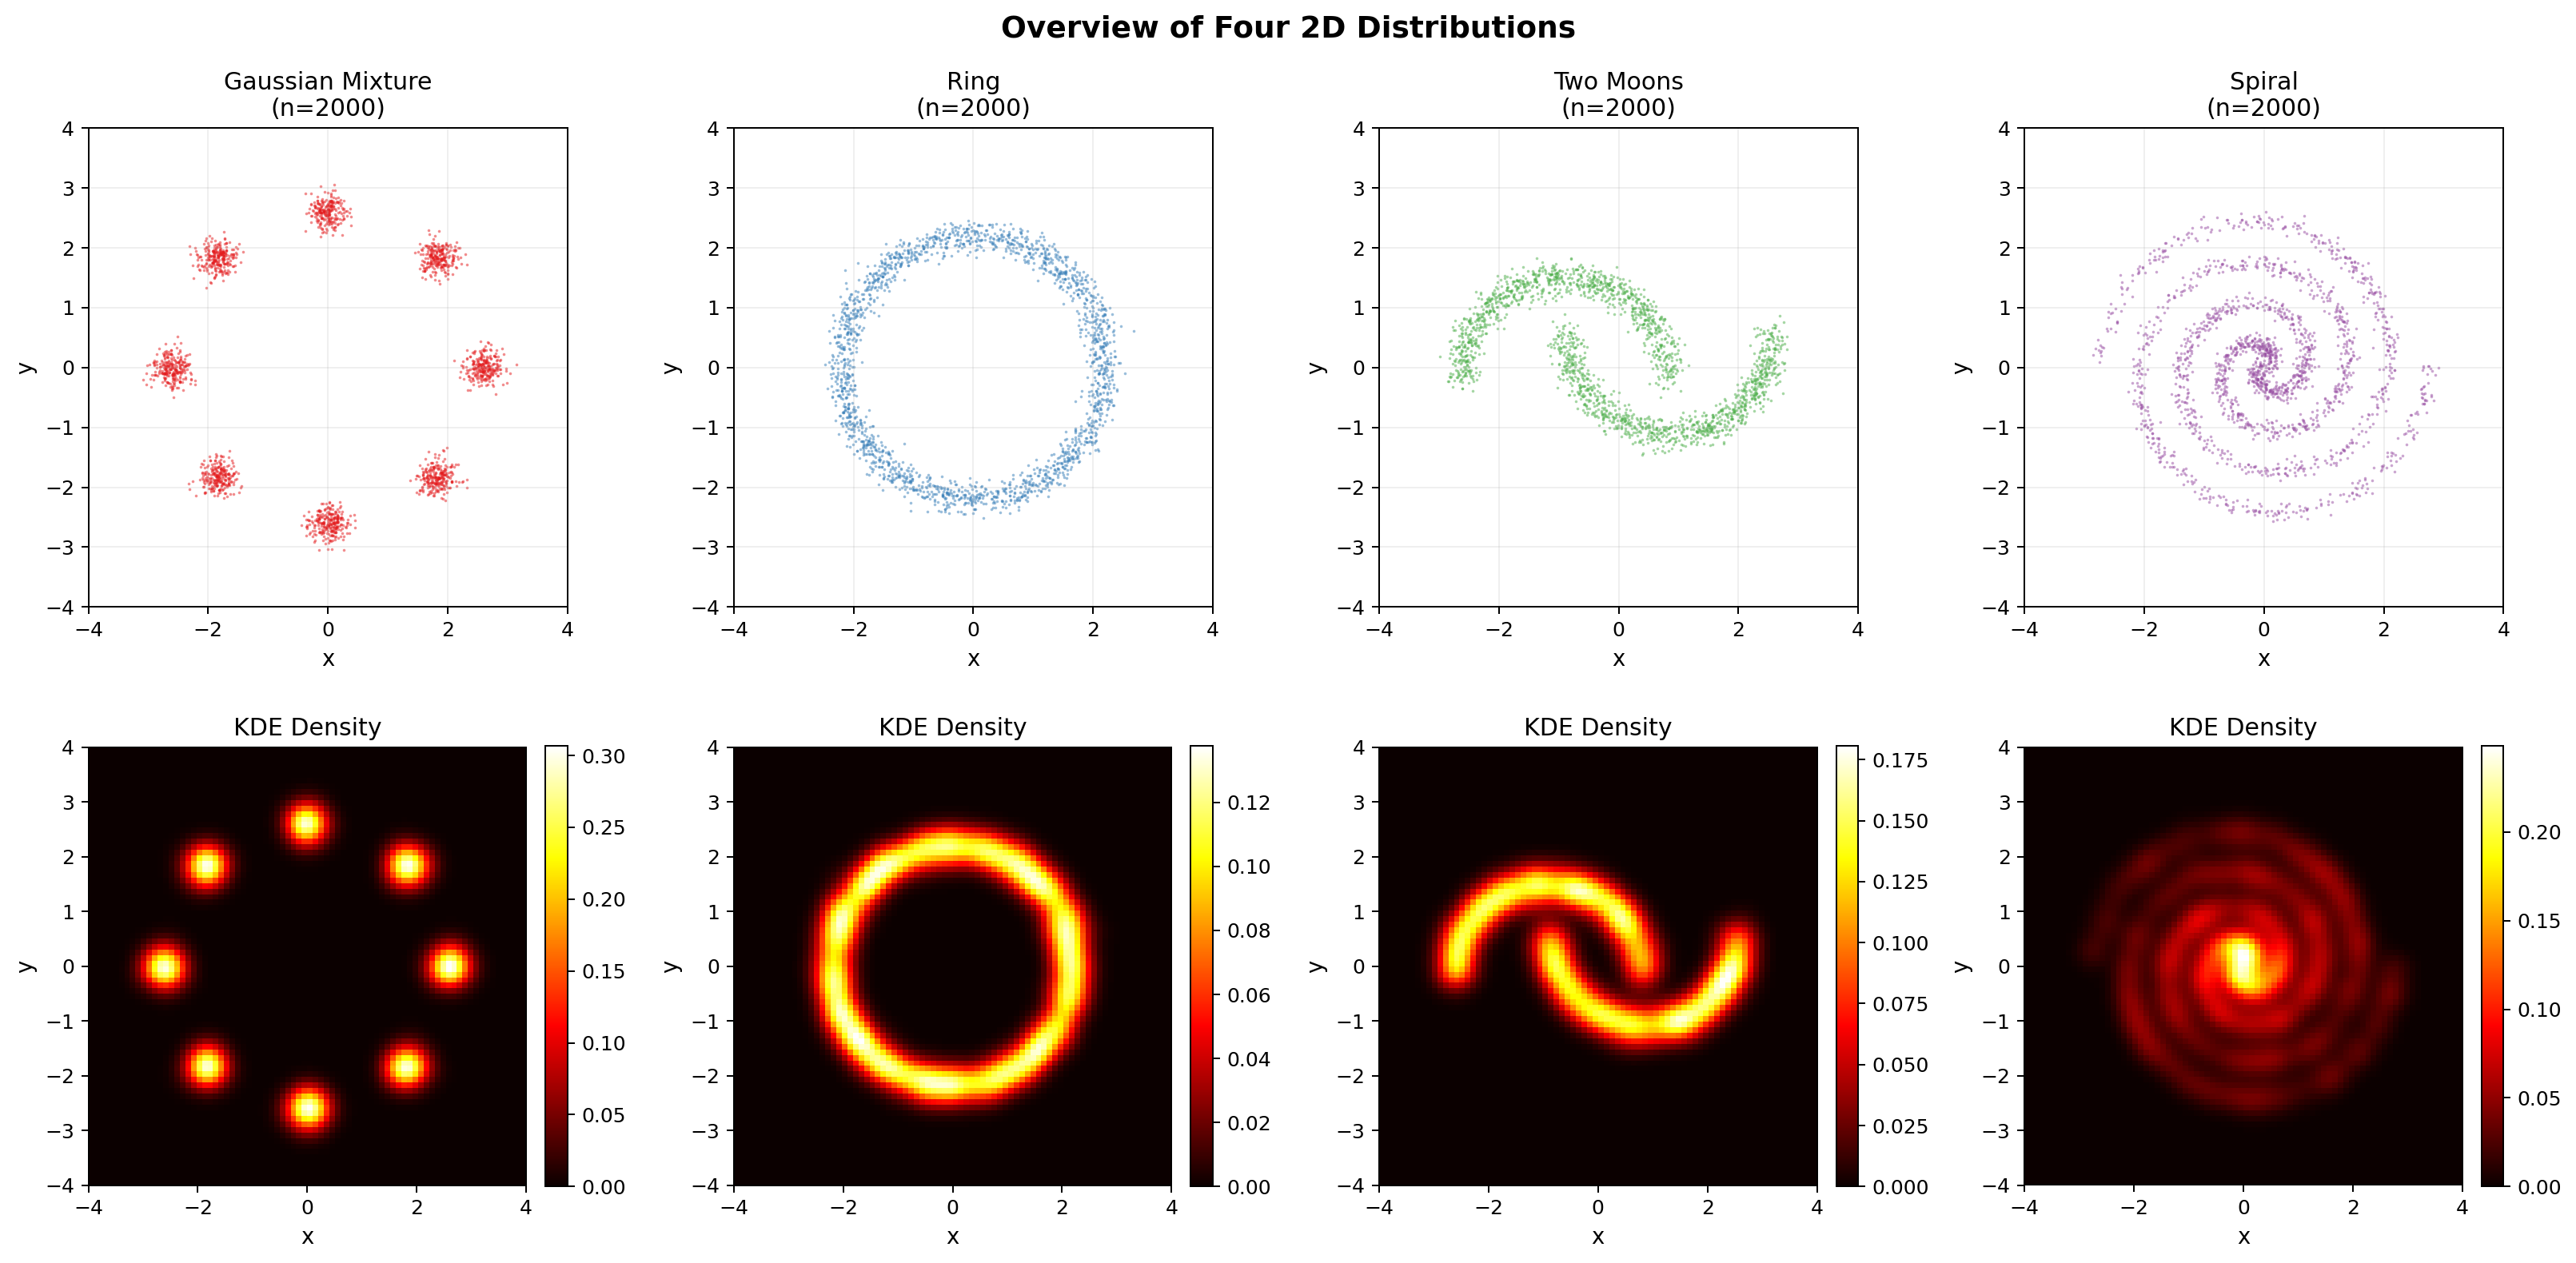
\includegraphics[width=0.90\textwidth]{comparison_overview.pdf}
    \caption{四类二维分布的散点图与 KDE 密度叠加图。颜色深浅表示经验密度，黑色等高线刻画主要支撑区域。}
    \label{fig:overview}
\end{figure}

\begin{figure}[!htbp]
    \centering
    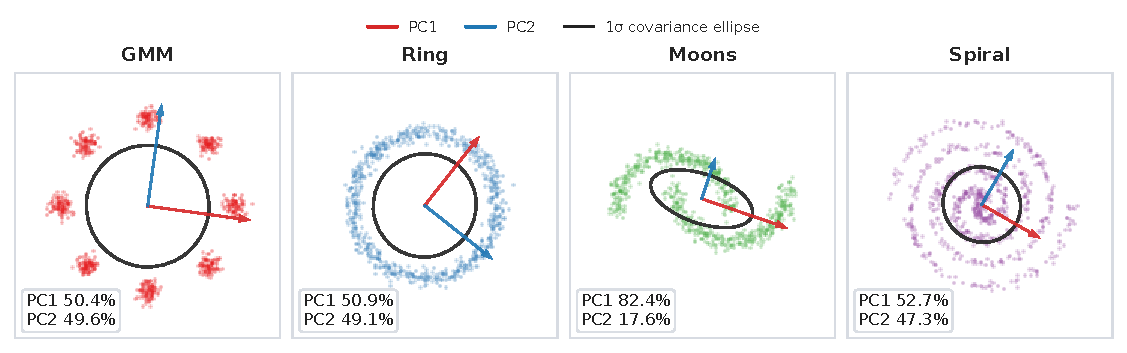
\includegraphics[width=0.90\textwidth]{pca_analysis.pdf}
    \caption{四类分布的 PCA 主方向与一倍标准差协方差椭圆。红色箭头表示第一主成分，蓝色箭头表示第二主成分。}
    \label{fig:pca}
\end{figure}

如图~\ref{fig:overview} 所示，四类二维分布呈现出截然不同的几何形态。Gaussian Mixture 代表了典型的离散多峰分布——概率密度集中在八个互不相连的团簇中，各团簇由低密度区域明确分隔。Ring、Two Moons 和 Spiral 构成非线性程度依次递增的低维连续流形——数据本质上依附于一维曲线，但以非线性的方式嵌入在二维观测空间中。KDE 密度热力图进一步直观展示了各类分布在真实空间中的概率密度过渡区域。

在深入分析结构之前，本研究首先检查训练集与测试集的同分布性：通过 $60\times 60$ 离散网格上的 KDE 密度估计，计算各类别的 Jensen-Shannon 散度，结果均在 $10^{-3}$ 量级，从经验上支持训练集与测试集来自同一分布的假设。

\subsection{几何结构分析}

图~\ref{fig:pca} 从线性视角揭示了四类分布的结构差异。Two Moons 是唯一 PCA 有效的分布（PC1 占 $82.4\%$，各向异性比 $4.70$），而 Ring 和 Spiral 的 PC1 与 PC2 占比接近 $50\%$——但 PCA 的失效本身就是一个重要结论：Ring 和 Spiral 本质为一维流形，只是线性投影无法发现非线性流形结构。

\begin{figure}[!htbp]
    \centering
    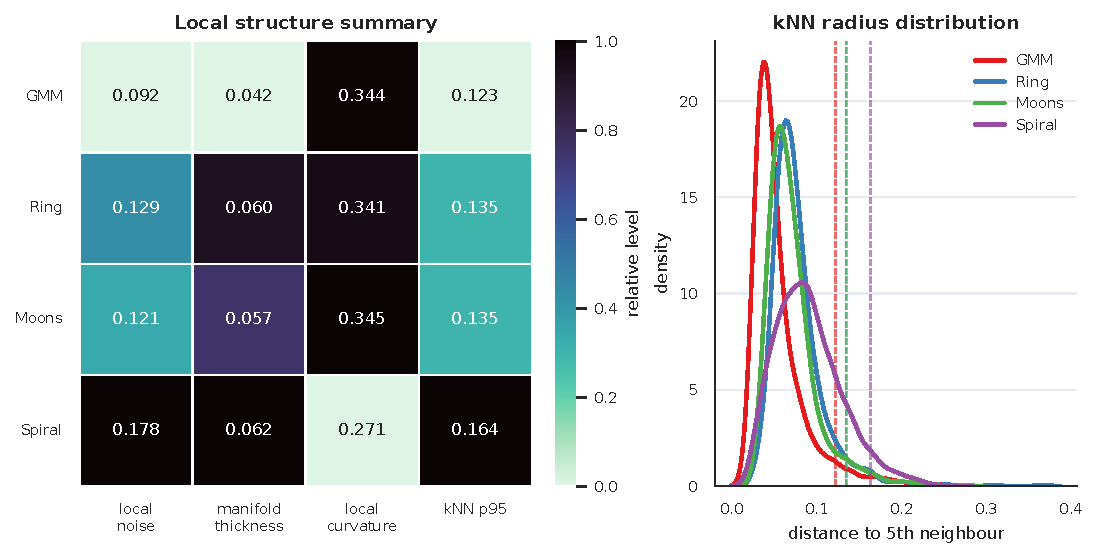
\includegraphics[width=0.90\textwidth]{noise_structure.pdf}
    \caption{局部结构统计摘要。左侧热力图给出局部噪声、流形厚度、局部曲率和 $k$-NN 半径的相对水平；右侧曲线展示第 5 近邻半径分布，虚线为 95\% 分位数。}
    \label{fig:noise}
\end{figure}

\begin{figure}[!htbp]
    \centering
    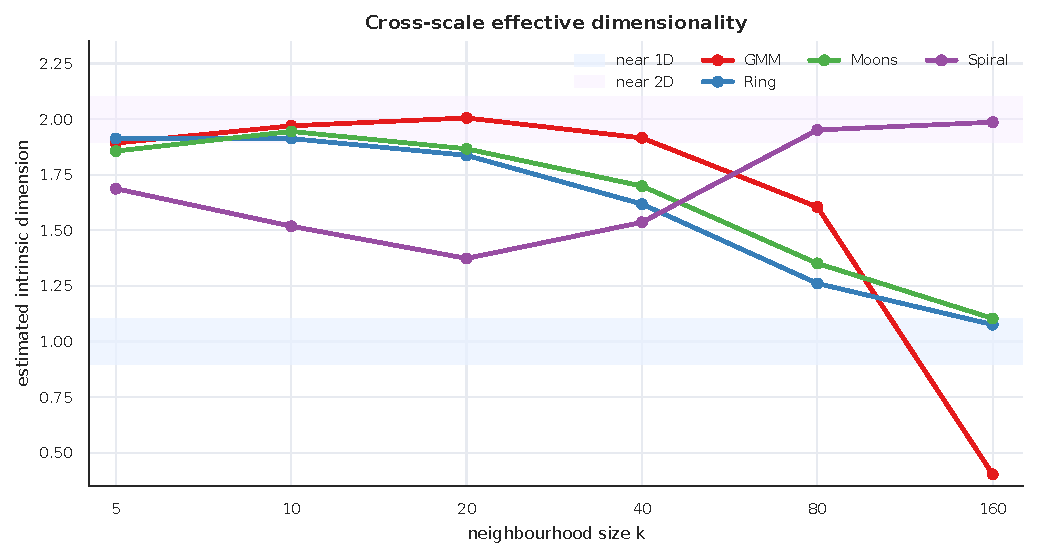
\includegraphics[width=0.86\textwidth]{effective_dimension.pdf}
    \caption{跨尺度有效维度估计。横轴为邻域规模 $k$，纵轴为基于 $k$-NN 半径比例估计的局部内在维度。}
    \label{fig:effdim}
\end{figure}

图~\ref{fig:noise} 和图~\ref{fig:effdim} 从噪声和维度的角度揭示了生成精度要求。Gaussian Mixture 各团簇厚度最小（$0.041$），团簇内部高度紧凑。Ring 在视觉上极薄（径向标准差 $0.13$），但局部厚度估计（$0.059$）反映的是环带径向宽度。Spiral 的厚度最大（$0.060$）且空间变化最为显著——外围噪声高达 $0.25$ 以上而内部仅约 $0.10$，体现沿径向递减的密度分布。跨尺度有效维度估计进一步说明：Gaussian Mixture 在小尺度上表现为二维团簇内部结构，但在大尺度上受模式间分离影响明显；Ring 与 Two Moons 随邻域尺度增大逐渐接近一维流形；Spiral 则在较大尺度上仍维持较高有效维度，反映其缠绕结构具有更强的全局复杂性。

\subsection{极坐标视角：拓扑结构的简化}

极坐标分析并非对所有分布都同等有效。本文仅对 Ring 和 Spiral 使用极坐标视角，是因为二者具有明确的径向--角向结构：Ring 近似满足 $r=\mathrm{const}$，其主要难点是保持闭合环带和中心空洞；Spiral 则近似满足 $r=f(\theta)$，其核心结构可以理解为相位推进过程中半径单调变化。相比之下，Gaussian Mixture 的多个团簇不共享自然极点，Two Moons 也不是关于原点的星形流形，强行转换到极坐标会引入坐标伪影，反而掩盖其多峰分离和非凸分支结构。因此，二者主要通过局部几何统计、有效维度和后续 Coverage--Precision 指标进行刻画。

\begin{figure}[!htbp]
    \centering
    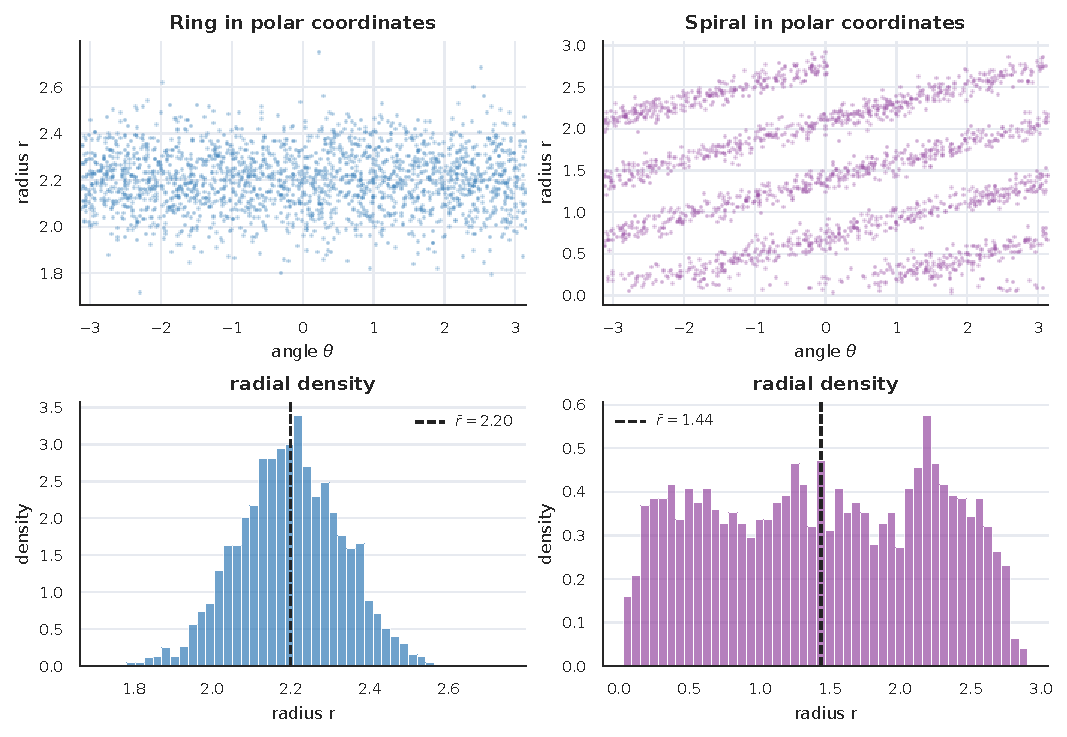
\includegraphics[width=0.78\textwidth]{polar_analysis.pdf}
    \caption{Ring与Spiral的极坐标$(r,\theta)$表示与径向分布$p(r)$直方图。}
    \label{fig:polar}
\end{figure}

图~\ref{fig:polar} 展示了坐标变换对拓扑结构的简化效果。Ring 在极坐标下塌缩为依附于 $r\approx 2.2$ 的高斯带（径向与角度相互独立），Spiral 的 $r$ 与 $\theta$ 呈线性依赖关系。这一拓扑等价变换具有深刻的理论启示：复杂数据分布可以通过一系列可逆的非线性映射，变换为易于采样的简单先验分布——这正是 Normalizing Flows 和扩散模型逆向过程的核心思想。

\subsection{分布几何难度画像}

为定量刻画四类分布的建模挑战，本文构建五个归一化几何维度：\textbf{局部噪声}表示样本到邻近点的平均距离，反映局部扰动强弱；\textbf{流形厚度}由局部 PCA 的最小方差方向估计，反映数据支撑集的横向宽度；\textbf{局部曲率}用邻域协方差特征值比例刻画，反映支撑集在小尺度上的弯曲程度；\textbf{PCA 非线性}衡量线性主成分解释能力的不足，数值越高说明越难用单一线性方向概括；\textbf{空间跨度}用平均两两距离近似，反映分布在观测空间中的展开范围。五个维度均在四类分布之间做 min--max 归一化，因此数值表示相对难度而非绝对物理量。

\begin{table}[!htbp]
\centering
\footnotesize
\caption{四类分布的几何特征与建模难点}
\label{tab:geo_features}
\begin{tabular*}{0.96\textwidth}{@{\extracolsep{\fill}}llll}
\toprule
分布 & 几何特征 & 建模难点 & 预期瓶颈指标 \\
\midrule
Gaussian Mixture & 离散多峰 & 模式覆盖与权重均衡 & Coverage, MMD \\
Ring & 闭合环形流形 & 中心空洞保持 & Precision, Coverage \\
Two Moons & 双非凸弧形流形 & 间隔保持与端点覆盖 & MMD, Wasserstein \\
Spiral & 高曲率缠绕流形 & 长程相位一致性 & MMD, Coverage, 视觉诊断 \\
\bottomrule
\end{tabular*}
\end{table}

\begin{figure}[!htbp]
    \centering
    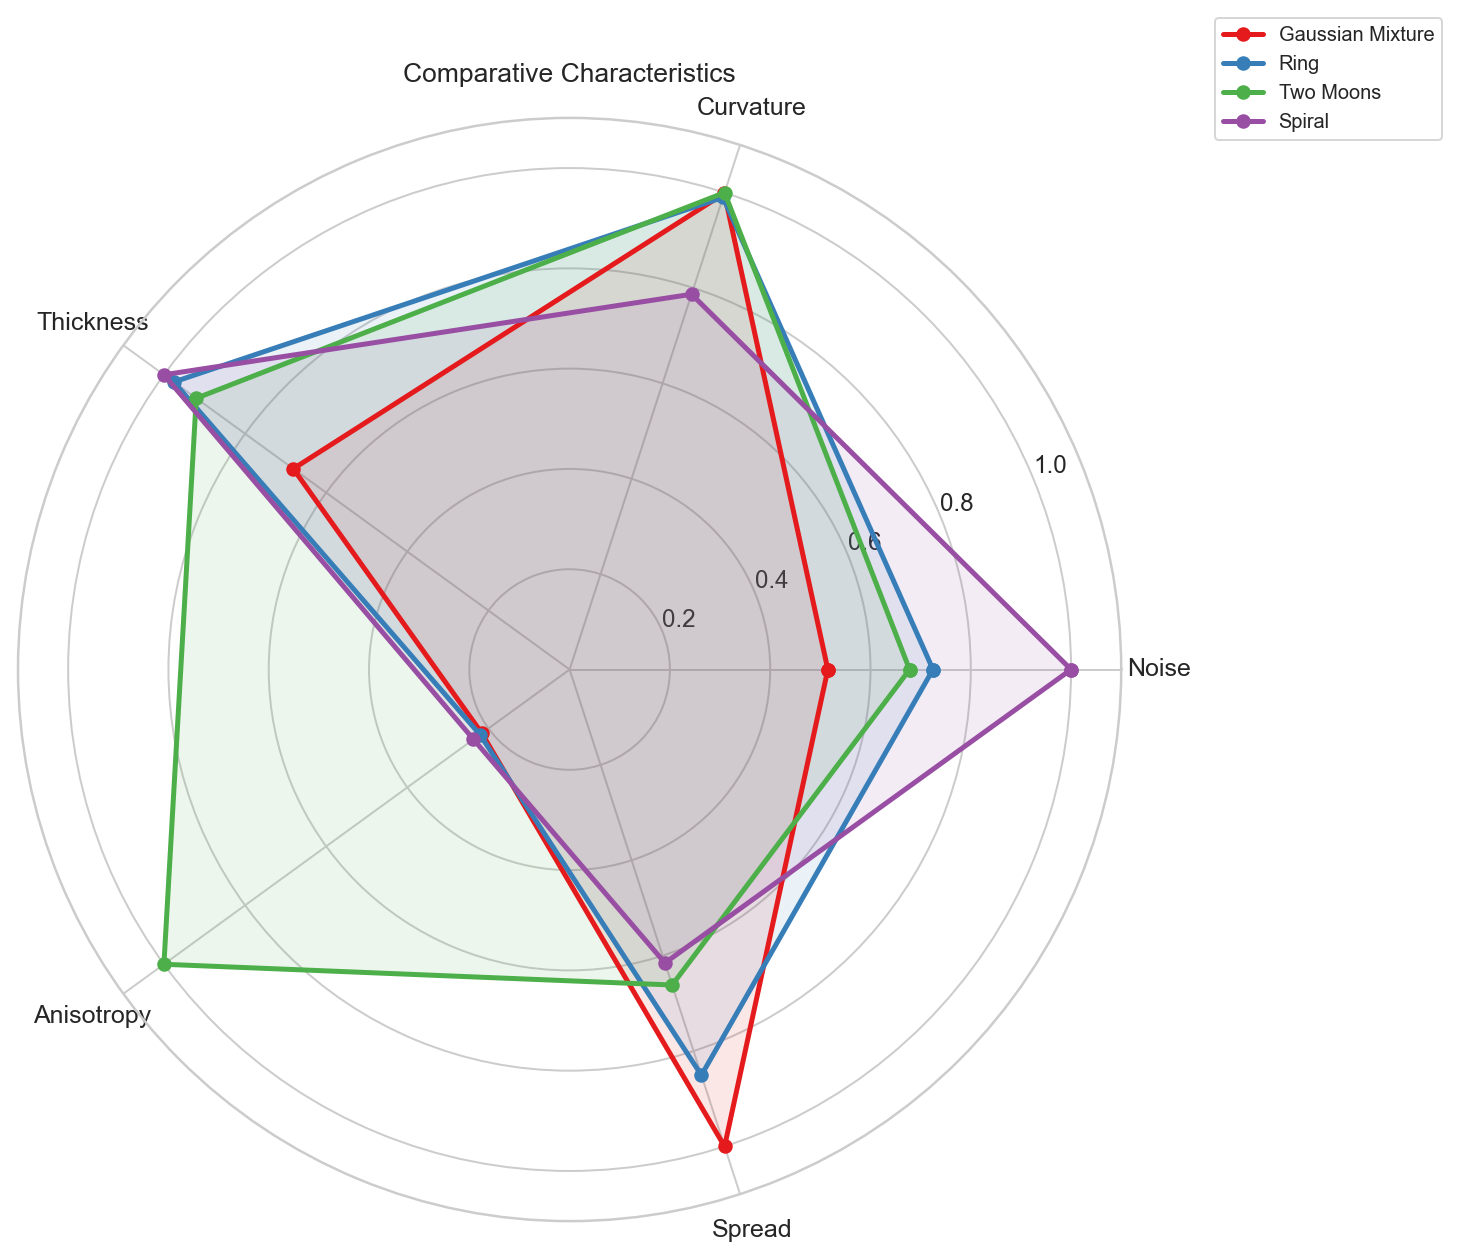
\includegraphics[width=0.58\textwidth]{summary_radar.pdf}
    \caption{四类分布在五个核心维度上的归一化几何难度画像。雷达图中半径 $0$ 表示该维度在四类中相对最低，半径 $1$ 表示相对最高；若某条边贴近中心，是因为该分布在对应维度上的归一化值接近 $0$，并非缺少维度。}
    \label{fig:difficulty_radar}
\end{figure}

综合以上分析，四类分布的建模难度呈现清晰的梯度：\textbf{Gaussian Mixture < Two Moons $\approx$ Ring < Spiral}。这一排序为后续实验设计提供了明确预期：Spiral 最可能暴露模型在全局结构表达上的差异，而 Ring 和 Two Moons 则更直接检验模型对薄流形与非凸支撑集的保持能力。

% ==================== 4. 生成模型建立 ====================
\section{生成模型建立}

本节详述 VAE 和 DDPM 两类深度生成模型的数学原理。前者基于 KL 散度的概率分布匹配，后者基于分数匹配的分步去噪，两者构成了两种截然不同的生成范式。

\subsection{变分自编码器（VAE）}

\subsubsection{概率建模与 ELBO 推导}

VAE \cite{kingma2014vae} 的核心思想是：假设数据 $\vect{x}\in\R^{2}$ 的生成过程受潜变量 $\vect{z}\in\R^{d}$ 支配——先从标准正态先验 $p(\vect{z})=\Ncal(0,\vect{I})$ 采样 $\vect{z}$，再通过参数化解码器 $p_{\theta}(\vect{x}\mid\vect{z})$ 生成数据。对任意观测样本，对数似然可写为：
\begin{equation}
    \log p_{\theta}(\vect{x}) = \log\int p_{\theta}(\vect{x}\mid\vect{z})\,p(\vect{z})\,\mathrm{d}\vect{z}
\end{equation}
该积分在一般情况下无闭式解。VAE 的关键创新是引入近似后验分布 $q_{\phi}(\vect{z}\mid\vect{x}) = \Ncal(\vect{\mu}_{\phi}(\vect{x}), \operatorname{diag}(\vect{\sigma}_{\phi}^2(\vect{x})))$，通过对数似然的 Jensen 下界得到证据下界（ELBO）：
\begin{equation}
    \log p_{\theta}(\vect{x}) \ge \underbrace{\E_{\vect{z}\sim q_{\phi}}[\log p_{\theta}(\vect{x}\mid\vect{z})]}_{\text{重构项}} - \underbrace{\KL\bigl(q_{\phi}(\vect{z}\mid\vect{x})\,\big\|\,p(\vect{z})\bigr)}_{\text{KL正则项}}
\end{equation}
采用 MSE 近似重构项并引入 KL 权重 $\beta$，得训练损失：
\begin{equation}
    \mathcal{L}_{\mathrm{VAE}}(\theta,\phi) = \E_{\vect{x}}\!\left[\norm{\vect{x} - \hat{\vect{x}}}^2 + \beta\cdot\frac{1}{2}\sum_{j=1}^{d}\bigl(\mu_j^2 + \sigma_j^2 - \log\sigma_j^2 - 1\bigr)\right]
\end{equation}

\subsubsection{重参数化技巧的数学本质}

ELBO 的梯度估计面临一个关键障碍：期望 $\E_{\vect{z}\sim q_{\phi}}$ 中的采样操作依赖于参数 $\phi$，构成不可微的随机节点，直接阻断梯度从解码器向编码器的反向传播。重参数化技巧将采样改写为确定性变换：
\begin{equation}
    \vect{z} = \vect{\mu}_{\phi}(\vect{x}) + \vect{\sigma}_{\phi}(\vect{x}) \odot \vect{\epsilon}, \qquad \vect{\epsilon}\sim\Ncal(0,\vect{I})
\end{equation}
随机性被隔离在外部变量 $\vect{\epsilon}$ 中（与 $\phi$ 无关），而 $\vect{z}$ 对 $\phi$ 的梯度可无阻碍传播：$\partial\vect{z}/\partial\vect{\mu}_{\phi}=\vect{I}$，$\partial\vect{z}/\partial\vect{\sigma}_{\phi}=\vect{\epsilon}$。数学本质上，重参数化是将随机计算图中的采样操作“提升”为可微的仿射变换。

\begin{figure}[!htbp]
    \centering
    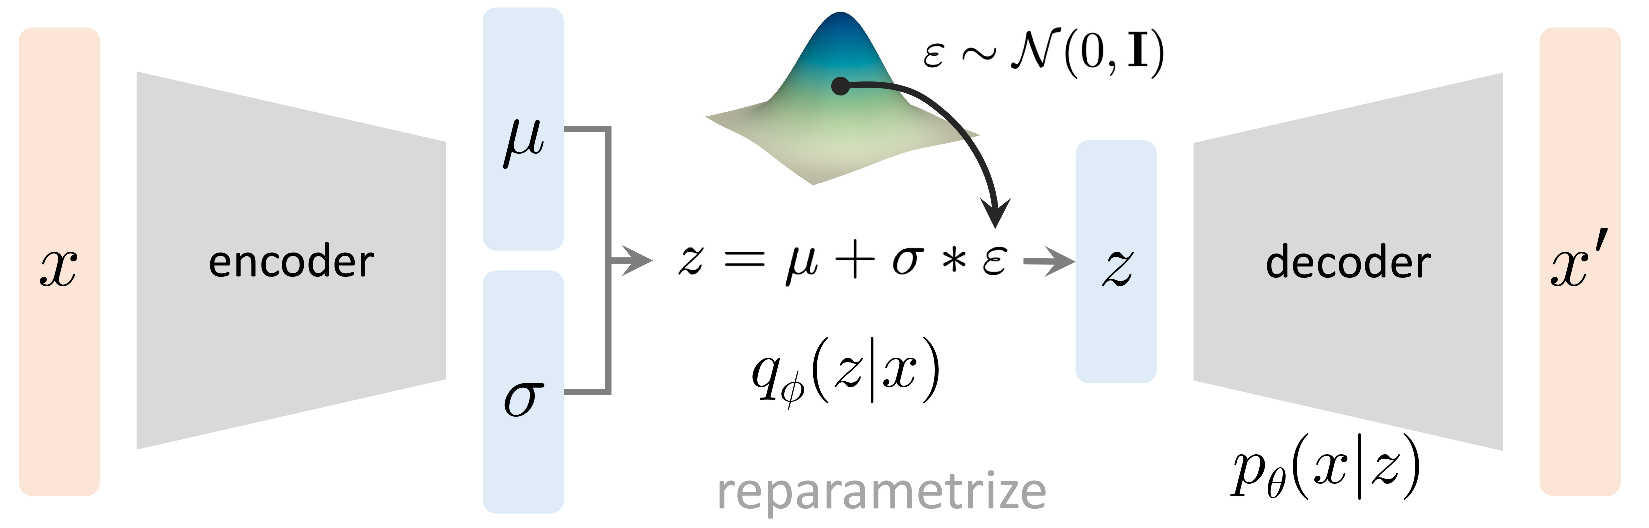
\includegraphics[width=0.85\textwidth]{vae.pdf}
    \caption{VAE 架构图：编码器输出潜分布参数$(\vect{\mu},\vect{\sigma})$，重参数化将采样可微化，解码器从潜变量重建数据。}
    \label{fig:vae_arch}
\end{figure}

\subsubsection{网络结构与训练细节}

本文 VAE 采用 MLP 骨干网络：编码器 $2\to128\to64\to8$（输出 $\vect{\mu}$ 和 $\log\vect{\sigma}^2$），解码器 $8\to64\to128\to2$。潜空间维度设为 $d=8$，为复杂流形提供充足表示容量的同时保持可解释性。优化器使用 Adam（学习率 $3\times 10^{-4}$）配合 Cosine 退火调度，共训练 800 个 epoch，批量大小 256，$\beta=1.0$。VAE 的优点在于训练稳定、采样速度快（单步前向约 $0.5\mathrm{ms}$）；缺点在于容易在高曲率或多流形交叉区域生成模糊的过渡样本——这是解码器连续映射的必要代价。

\subsection{去噪扩散概率模型（DDPM）}

\subsubsection{马尔可夫链拓扑与双向轨迹}

DDPM \cite{ho2020ddpm} 将生成过程建模为一条跨越 $T$ 个时间步的双向马尔可夫链，构建状态序列：
\begin{equation}
    \vect{x}_0 \;\leftrightarrow\; \vect{x}_1 \;\leftrightarrow\; \vect{x}_2 \;\leftrightarrow\; \cdots \;\leftrightarrow\; \vect{x}_T
\end{equation}
\textbf{前向加噪轨迹}（Diffusion Process）：从左向右运行，是固定、无参数的马尔可夫链。每步注入少量高斯噪声：
\begin{equation}
    q(\vect{x}_t\mid\vect{x}_{t-1}) = \Ncal\bigl(\sqrt{1-\beta_t}\,\vect{x}_{t-1},\; \beta_t\vect{I}\bigr)
\end{equation}
由高斯封闭性，任意 $\vect{x}_t$ 可直接从 $\vect{x}_0$ 表达：
\begin{equation}
    \vect{x}_t = \sqrt{\bar{\alpha}_t}\,\vect{x}_0 + \sqrt{1-\bar{\alpha}_t}\,\vect{\epsilon}, \quad \vect{\epsilon}\sim\Ncal(0,\vect{I})
\end{equation}
其中 $\alpha_t = 1-\beta_t$，$\bar{\alpha}_t = \prod_{s=1}^{t}\alpha_s$。随 $t$ 增大，$\bar{\alpha}_t\to 0$，结构化信息逐渐被高斯噪声淹没，最终 $\vect{x}_T\sim\Ncal(0,\vect{I})$。

\textbf{反向去噪轨迹}（Generative Process）：从右向左运行，是参数化的生成过程。DDPM 训练噪声预测网络 $\vect{\epsilon}_{\theta}(\vect{x}_t,t)$，优化简洁的 MSE 目标：
\begin{equation}
    \mathcal{L}_{\mathrm{DDPM}}(\theta) = \E_{t,\vect{x}_0,\vect{\epsilon}}\!\left[\norm{\vect{\epsilon} - \vect{\epsilon}_{\theta}\bigl(\sqrt{\bar{\alpha}_t}\,\vect{x}_0 + \sqrt{1-\bar{\alpha}_t}\,\vect{\epsilon},\;t\bigr)}^2\right]
\end{equation}
采样从纯噪声 $\vect{x}_T\sim\Ncal(0,\vect{I})$ 出发，逐步反向迭代 $t=T-1,\dots,0$：
\begin{equation}
    \vect{x}_{t-1} = \frac{1}{\sqrt{\alpha_t}}\Bigl(\vect{x}_t - \frac{\beta_t}{\sqrt{1-\bar{\alpha}_t}}\vect{\epsilon}_{\theta}(\vect{x}_t,t)\Bigr) + \sqrt{\beta_t}\,\vect{z}, \quad \vect{z}\sim\Ncal(0,\vect{I})\;(t>0)
\end{equation}

与 VAE 的单步生成不同，DDPM 的训练目标 $\mathcal{L}_{\mathrm{DDPM}}$ 经由时间步 $t$ 的均匀采样被分解为从 $t=0$（几乎无噪声）到 $t=T$（纯噪声）的连续谱——每个 $t$ 级别的去噪子任务只关注该噪声水平对应的特征尺度。高噪声水平处理全局粗粒度结构，低噪声水平精修局部细粒度结构，形成从粗到细的分层生成策略。这种“分而治之”的策略使 DDPM 在复杂几何结构上具有较强的建模适应性。

\begin{figure}[!htbp]
    \centering
    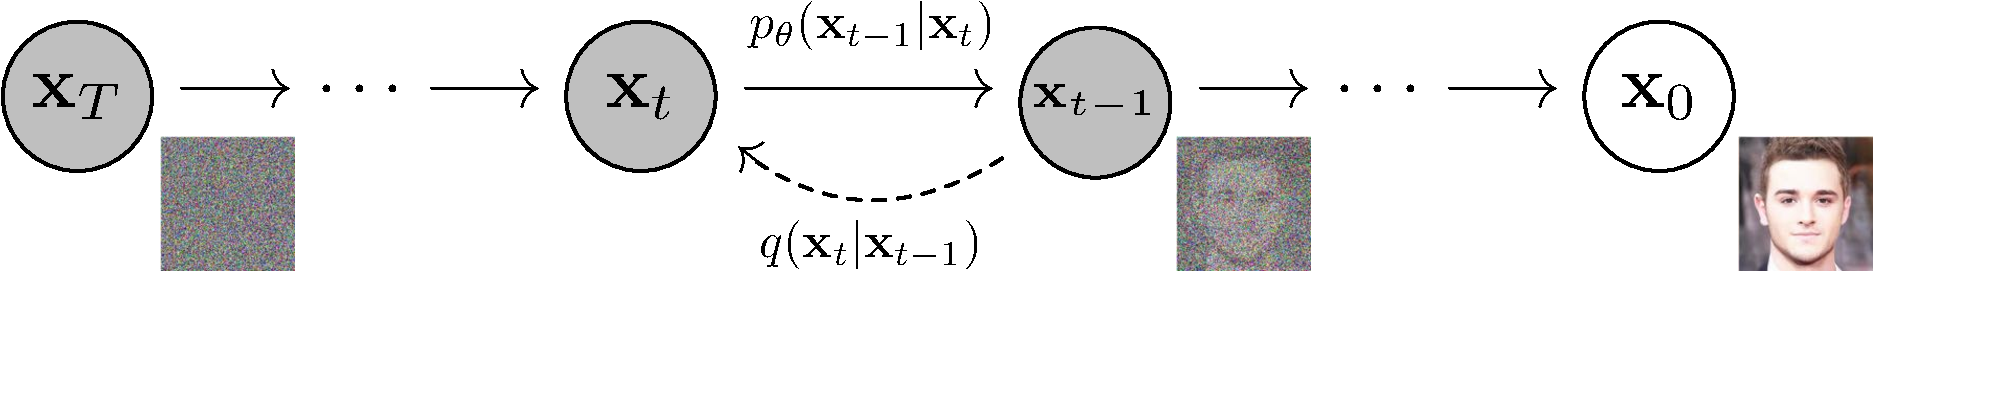
\includegraphics[width=0.90\textwidth]{ddpm.pdf}
    \caption{DDPM的双向马尔可夫链架构：前向加噪轨迹（自左向右）将数据$\vect{x}_0$逐步退化为纯噪声$\vect{x}_T$；反向去噪生成轨迹（自右向左）从噪声中逐步恢复结构化样本。}
    \label{fig:ddpm_arch}
\end{figure}

\subsubsection{网络结构与训练细节}

本文 DDPM 采用线性噪声调度（$\beta_t$ 从 $10^{-4}$ 线性增长至 $0.02$），$T=1000$。噪声预测网络以正弦时间嵌入（64 维）为条件，4 层 MLP（隐藏维度 256，ReLU 激活），输出 2 维噪声预测。优化器使用 Adam（学习率 $2\times 10^{-4}$），共训练 1500 个 epoch，批量大小 256。DDPM 的优点在于分布覆盖能力强、适合复杂非线性流形；缺点在于采样需执行完整的 $T$ 步迭代（约 $25\mathrm{ms}$），速度显著慢于单步方法。

% ==================== 5. 实验设计与样本生成 ====================
\section{实验设计与样本生成}

\subsection{数据划分与预处理}

本文直接采用课程提供的统一数据生成脚本。四类二维分布各包含 2000 个训练样本和 2000 个测试样本，所有样本坐标均位于 $[-4,4]\times[-4,4]$ 范围内。数据使用固定的随机种子（seed=42 和 seed=43）生成，训练集与测试集来自相同的分布但使用不同的随机种子以保证同分布性。

四类分布构成的难度梯度为：
\begin{enumerate}[label=(\arabic*)]
    \item \textbf{Gaussian Mixture}：8 个各向同性高斯团簇（中心在半径 $2.6$ 的圆上，$\sigma=0.16$）。考察模型的模式覆盖能力。
    \item \textbf{Ring}：闭合圆环（半径 $2.2$，径向噪声 $\sigma_r=0.13$，切向噪声 $\sigma_t=0.03$）。考察模型的拓扑保持能力。
    \item \textbf{Two Moons}：两段对称弯曲弧形（仿射变换：缩放 $1.75$，平移 $(-0.9,-0.25)$，噪声 $\sigma=0.08$）。考察模型的局部几何分辨能力。
    \item \textbf{Spiral}：两条阿基米德螺旋臂（$t\sim\mathcal{U}(0.25,4\pi)$，$r=0.22t$，相位差 $\pi$，噪声 $\sigma=0.08$）。考察模型的全局一致性。
\end{enumerate}

\subsection{模型训练设置}

两类模型在 NVIDIA GeForce RTX 4080 Laptop GPU（12GB 显存）上完成训练，软件环境为 PyTorch 2.7.0 + CUDA 12.6。详见表~\ref{tab:training_config}。

\begin{table}[!htbp]
\centering
\small
\caption{两类模型的训练配置}
\label{tab:training_config}
\begin{tabular*}{0.96\textwidth}{@{\extracolsep{\fill}}lll}
\toprule
配置项 & VAE & DDPM \\
\midrule
骨干网络 & MLP $(2,128,64,8,64,128,2)$ & Time-MLP, 4层, $h=256$ \\
参数量 & $\approx3.5\times10^4$ & $\approx2.0\times10^5$ \\
关键超参数 & $d_z=8,\ \beta=1.0$ & $T=1000,\ \beta_t:10^{-4}\to0.02$ \\
优化器 & Adam, $\mathrm{lr}=3\times10^{-4}$, cosine & Adam, $\mathrm{lr}=2\times10^{-4}$ \\
训练轮数 & 800 & 1500 \\
批量大小 & 256 & 256 \\
\bottomrule
\end{tabular*}
\end{table}

\subsection{生成样本直观比较}

\begin{figure}[!htbp]
    \centering
    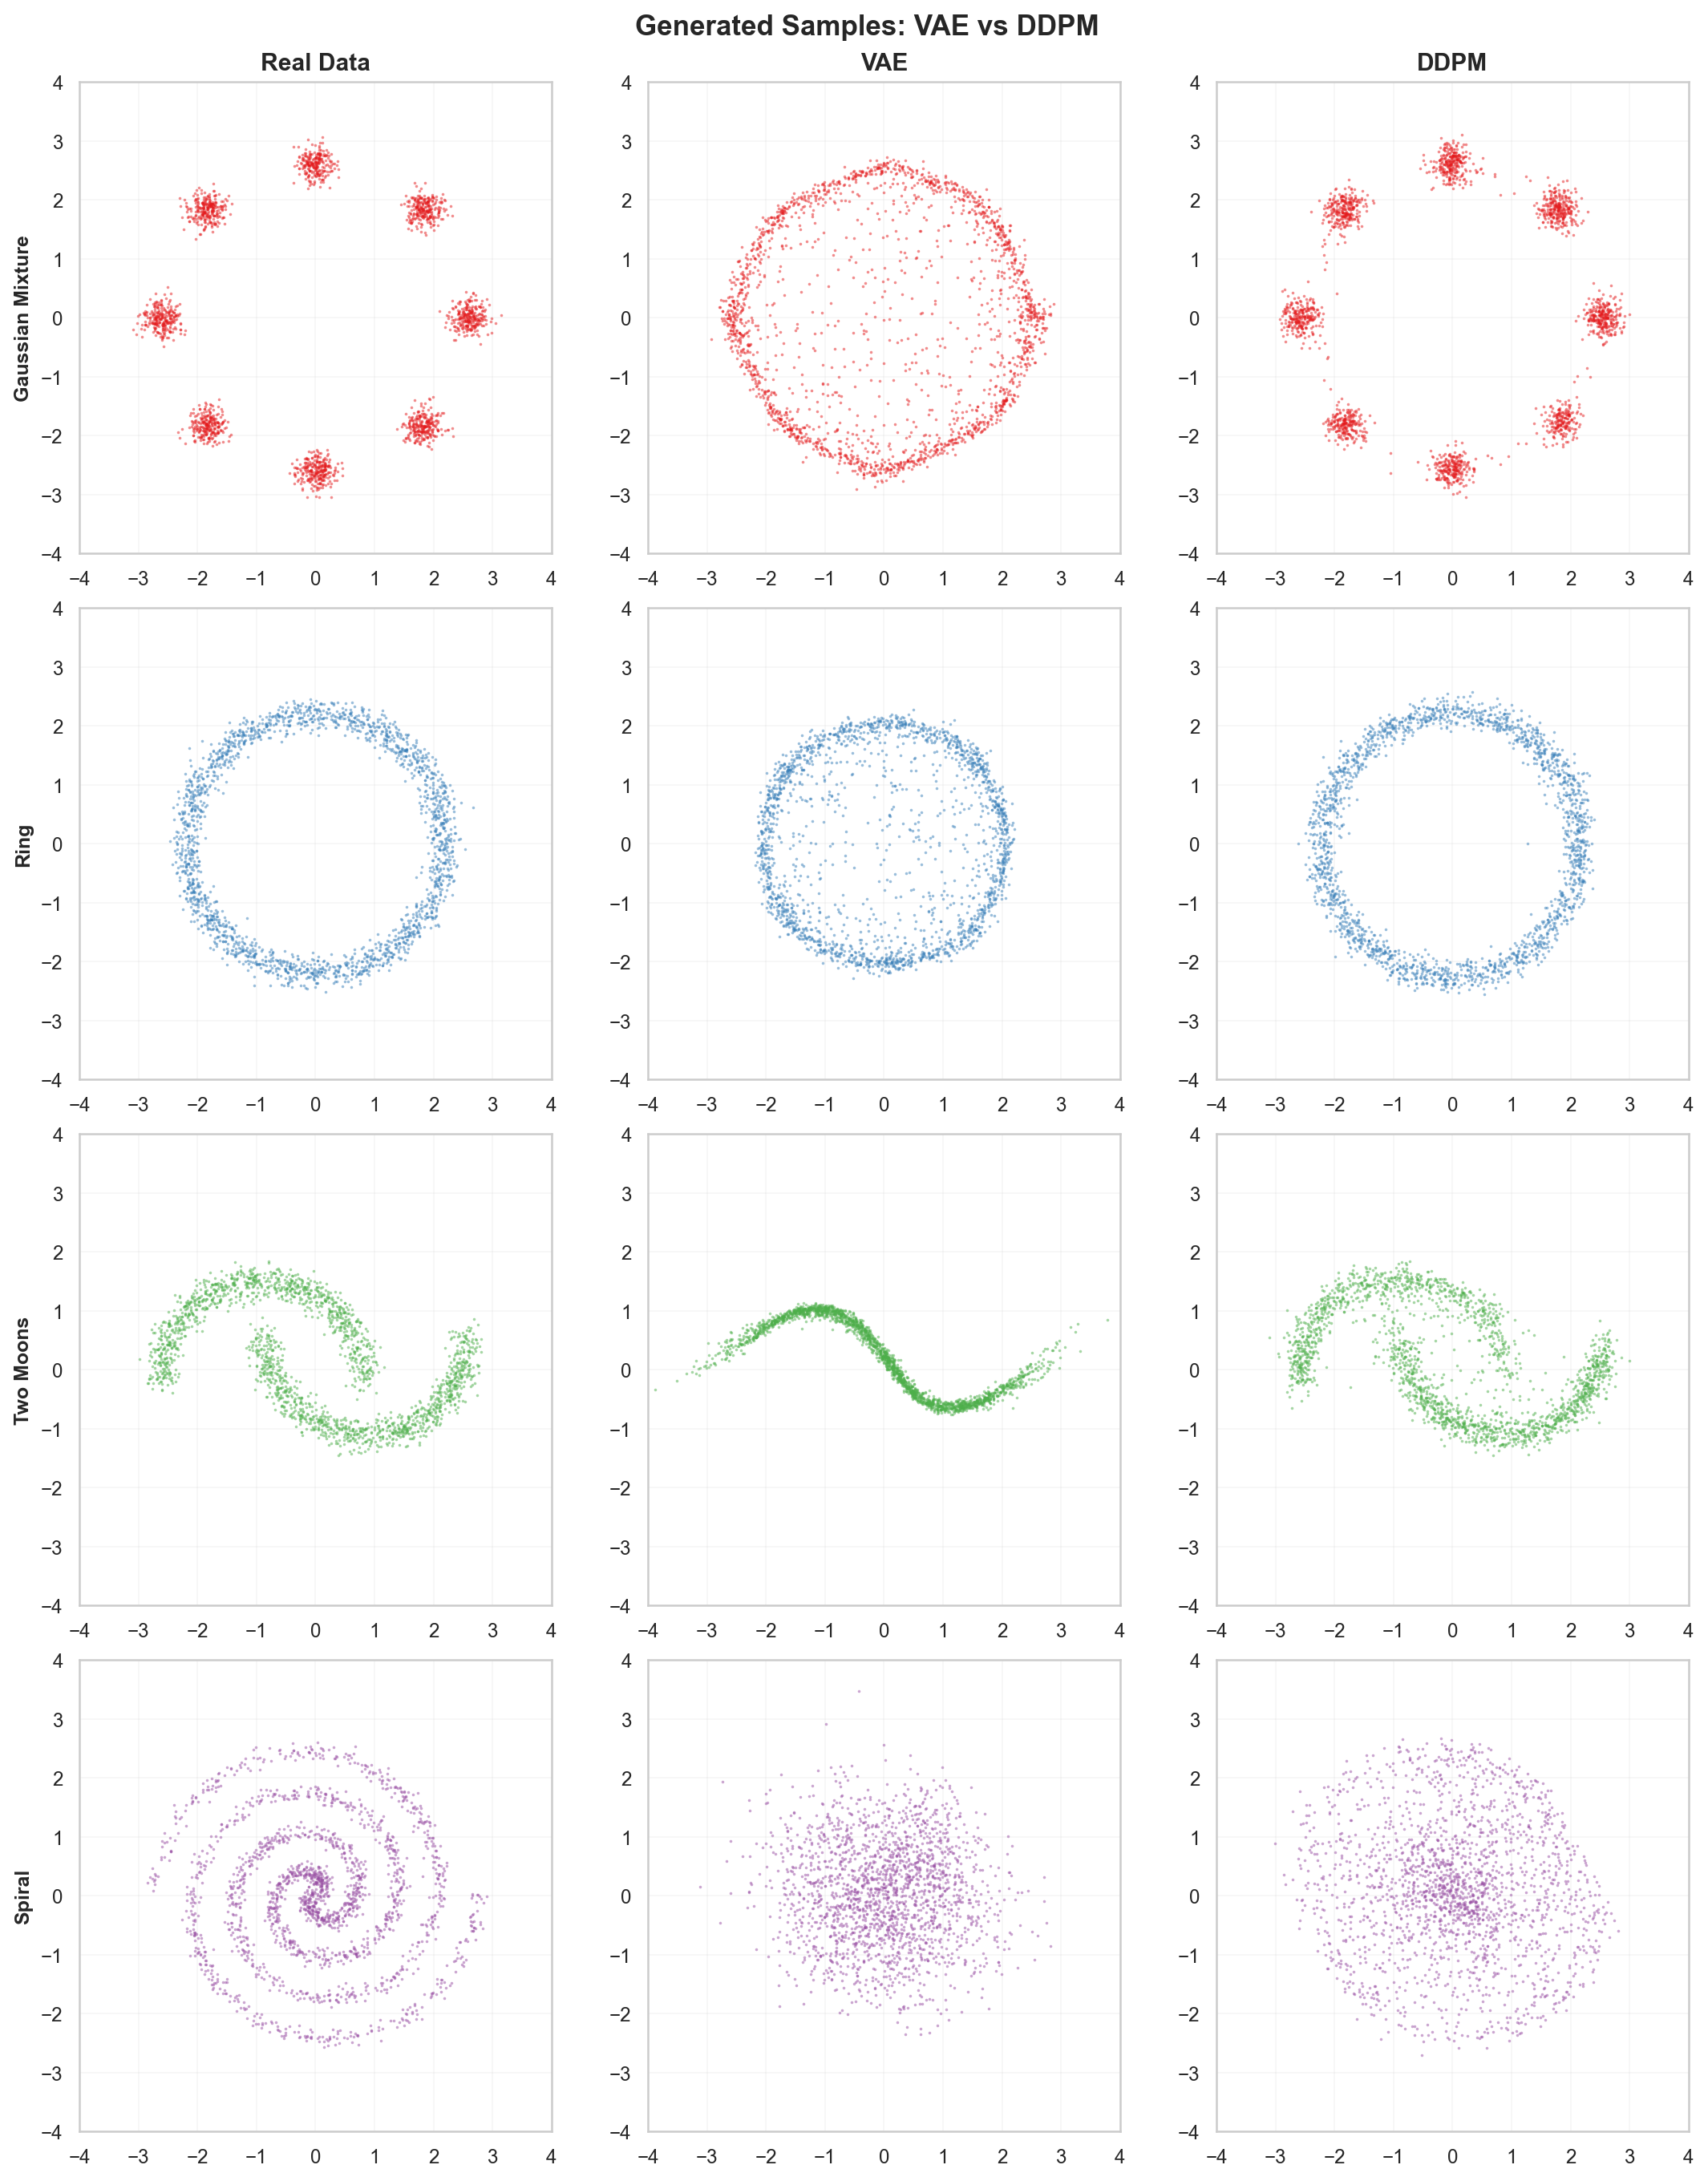
\includegraphics[width=0.92\textwidth]{generation_comparison.pdf}
    \caption{真实分布与生成分布的 KDE 等高线叠加对比。灰色为真实训练集密度，蓝色虚线为 VAE 生成分布，橙色实线为 DDPM 生成分布。}
    \label{fig:gen}
\end{figure}

图~\ref{fig:gen} 给出了两类模型生成样本与真实训练样本的直接视觉对比。Gaussian Mixture：DDPM 生成 8 个清晰分离的团簇，VAE 边界模糊且团簇间有“桥接”样本——解码器在接收到相邻潜变量时输出两者的均值位置。Ring：DDPM 环带最薄最均匀，VAE 环带厚 $1.5$--$2$ 倍——单步解码的平滑化效应将薄环“涂厚”。Two Moons：DDPM 准确保持两弧之间的狭窄间隔，VAE 在两弧端点处样本混杂。Spiral：DDPM 保持双螺旋宏观形态，VAE 出现明显的“团化”和“增厚”。

\subsection{扩散去噪过程可视化}

\begin{figure}[!htbp]
    \centering
    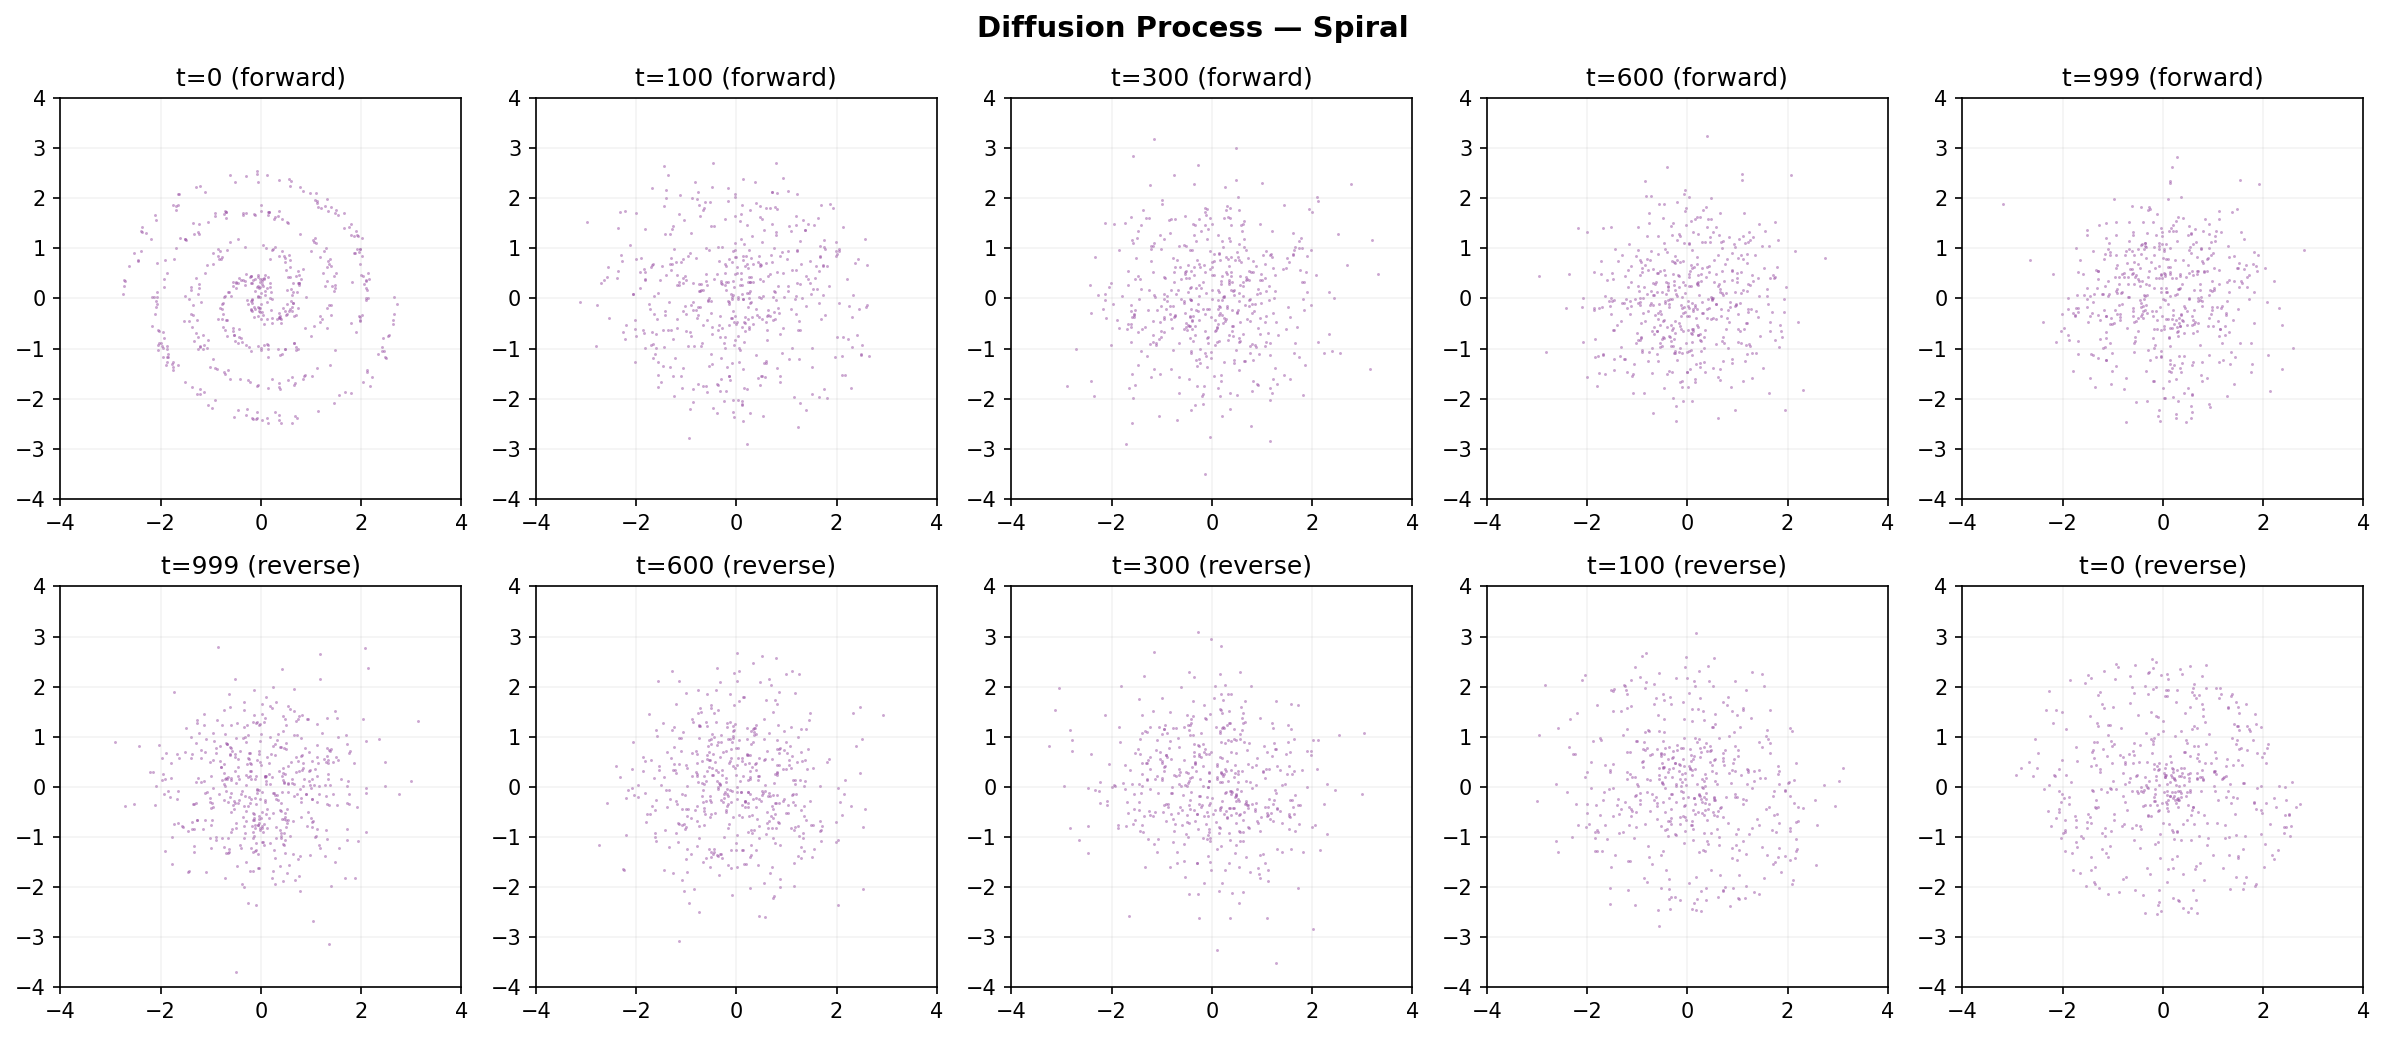
\includegraphics[width=0.92\textwidth]{diffusion_process.pdf}
    \caption{DDPM在Ring上的前向扩散（上排，$t=0\to999$）与反向去噪（下排，$t=999\to0$）过程。}
    \label{fig:diffusion}
\end{figure}

图~\ref{fig:diffusion} 展示了 DDPM 从纯噪声逐步恢复环形支撑集的过程。前向加噪展示了闭合环结构在噪声注入中的逐级丢失；反向去噪则展现了“从无序中恢复结构”：高噪声阶段先形成粗略的全局轮廓，低噪声阶段进一步压缩到薄环附近并保持中心空洞。这一可视化直接印证了 DDPM 分步去噪的多尺度机制——高噪声水平处理全局轮廓，低噪声水平精修局部细节——正是这种机制赋予了 DDPM 处理复杂流形的局部几何优势。

\subsection{训练收敛曲线}

\begin{figure}[!htbp]
    \centering
    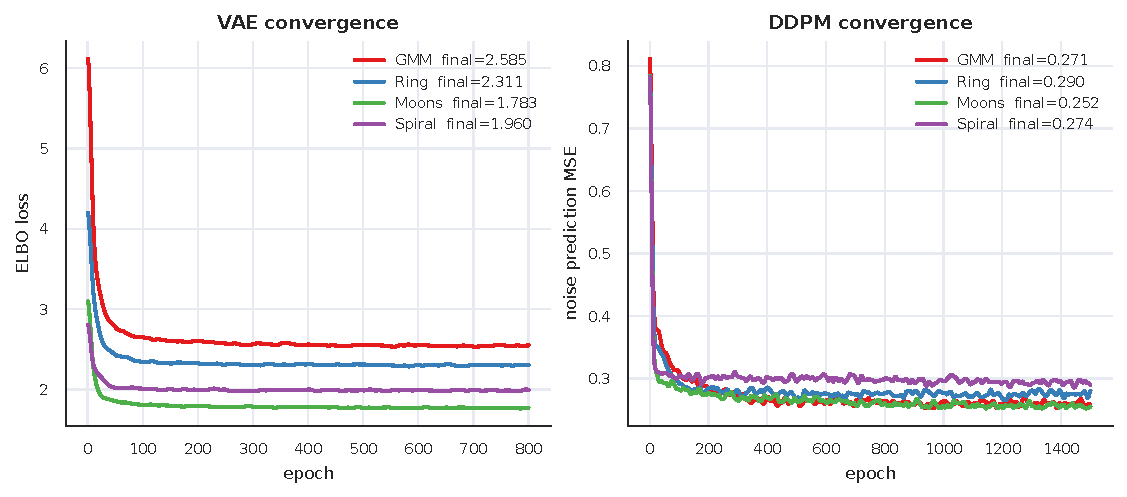
\includegraphics[width=0.92\textwidth]{training_curves.pdf}
    \caption{VAE 与 DDPM 在四类分布上的训练收敛曲线。左图为 VAE 的 ELBO 损失，右图为 DDPM 的噪声预测均方误差。}
    \label{fig:training}
\end{figure}

图~\ref{fig:training} 展示了训练收敛过程。VAE 的 ELBO 在约 $400$--$600$ epoch 后趋于平稳，最终损失与分布复杂度正相关：Two Moons（$1.78$）< Spiral（$1.96$）< Ring（$2.31$）< Gaussian Mixture（$2.59$）。DDPM 的 MSE 在所有分布上稳定收敛至 $0.25$--$0.29$ 的窄区间，跨分布标准差仅 $0.015$——无论数据是团簇还是螺旋，预测高斯噪声这一训练子任务的数值难度相近，但这并不意味着最终采样质量对几何结构完全不敏感。

% ==================== 6. 生成质量评价 ====================
\section{生成质量评价}

\subsection{最大均值差异（MMD）}

MMD \cite{gretton2012mmd} 衡量两组样本在再生核希尔伯特空间中均值嵌入的距离。对于真实样本集 $X$ 和生成样本集 $Y$：
\begin{equation}
    \operatorname{MMD}^2(X,Y) = \frac{1}{|X|^2}\sum_{i,j}k(\vect{x}_i,\vect{x}_j) + \frac{1}{|Y|^2}\sum_{i,j}k(\vect{y}_i,\vect{y}_j) - \frac{2}{|X||Y|}\sum_{i,j}k(\vect{x}_i,\vect{y}_j)
\end{equation}
本文采用 RBF 核 $k(\vect{x},\vect{y}) = \exp(-\norm{\vect{x}-\vect{y}}^2/2\sigma^2)$，带宽 $\sigma$ 通过样本中位数距离自动选取。MMD 越小表示生成分布与真实分布在整体统计意义上越接近。注意 MMD 主要反映全局分布匹配，对局部几何细节的分辨力有限。

\subsection{Wasserstein 距离}

Wasserstein 距离基于最优传输理论，衡量将一个分布“搬运”到另一个分布的最小几何代价。本文采用熵正则化 Sinkhorn 算法 \cite{rabin2011swd}：对真实集 $X$ 和生成集 $Y$ 各随机抽取 $500$ 个点，构建代价矩阵 $C_{ij}=\norm{\vect{x}_i-\vect{y}_j}^2$（归一化后），正则化参数 $\varepsilon=0.01$。Wasserstein 距离对支撑集的几何形状差异高度敏感——如果生成样本的支撑集与真实数据的支撑集在形状上有系统性偏移，该指标会显著响应。

\subsection{Coverage 与 Precision}

Coverage 和 Precision \cite{kyukaaniemi2019prdc} 基于 $k$-NN（$k=5$）流形半径定义，从样本级别揭示互补的生成质量信息：
\begin{align}
    \operatorname{Coverage} &= \frac{1}{|X|}\sum_{\vect{x}\in X} \mathbf{1}\!\left[\min_{\hat{\vect{x}}\in \hat{X}}\norm{\vect{x} - \hat{\vect{x}}} < r_k(\vect{x},X)\right] \\
    \operatorname{Precision} &= \frac{1}{|\hat{X}|}\sum_{\hat{\vect{x}}\in \hat{X}} \mathbf{1}\!\left[\min_{\vect{x}\in X}\norm{\hat{\vect{x}} - \vect{x}} < \operatorname{percentile}_{95}(r_k(\cdot,X))\right]
\end{align}
Coverage 衡量“有多全”——真实样本中被至少一个生成样本覆盖的比例。Precision 衡量“有多真”——生成样本中落在真实流形内的比例。两者互补：高 Precision 伴随低 Coverage 指示模式坍塌，低 Precision 伴随高 Coverage 暗示生成样本虽分布广但质量粗糙。这种互补的诊断能力使其成为诊断生成模型失效模式的理想工具。

\subsection{综合得分}

为直观展示模型排序，将各指标归一化为“越大越好”并加权求和。对于 MMD 和 Wasserstein 等越小越好的指标，取 $s_j = 1 - (m_j - m_j^{\min}) / (m_j^{\max} - m_j^{\min})$；对 Precision 和 Coverage 等越大越好的指标，取 $s_j = (m_j - m_j^{\min}) / (m_j^{\max} - m_j^{\min})$。赋予四项指标等权 $w_j = 0.25$，定义综合得分：
\begin{equation}
    S = \sum_{j} w_j \cdot s_j
\end{equation}
综合得分仅用于整体排序，不替代单项指标的具体分析。

\subsection{定量评价结果}

\begin{table}[!htbp]
\centering
\small
\caption{两类模型在各分布上的生成质量评价结果（粗体为最优值）}
\label{tab:main_results}
\begin{tabular}{llccccc}
\toprule
分布 & 模型 & MMD$\downarrow$ & Wass.$\downarrow$ & Cov.$\uparrow$ & Prec.$\uparrow$ & 综合得分$\uparrow$ \\
\midrule
\multirow{2}{*}{Gaussian Mixture}
    & VAE   & \textbf{0.0033} & \textbf{0.132} & 0.552 & 0.475 & 0.387 \\
    & DDPM  & 0.0040 & 0.151 & \textbf{0.963} & \textbf{0.966} & \textbf{0.666} \\
\midrule
\multirow{2}{*}{Ring}
    & VAE   & 0.0047 & 0.116 & 0.664 & 0.806 & 0.619 \\
    & DDPM  & \textbf{0.0002} & \textbf{0.095} & \textbf{0.972} & \textbf{0.992} & \textbf{0.969} \\
\midrule
\multirow{2}{*}{Two Moons}
    & VAE   & 0.0141 & 0.111 & 0.176 & 0.536 & 0.186 \\
    & DDPM  & \textbf{0.0010} & \textbf{0.087} & \textbf{0.968} & \textbf{0.966} & \textbf{0.972} \\
\midrule
\multirow{2}{*}{Spiral}
    & VAE   & 0.0098 & 0.115 & 0.777 & \textbf{0.976} & 0.649 \\
    & DDPM  & \textbf{0.0043} & \textbf{0.104} & \textbf{0.847} & \textbf{0.976} & \textbf{0.813} \\
\bottomrule
\end{tabular}
\end{table}

\begin{figure}[!htbp]
    \centering
    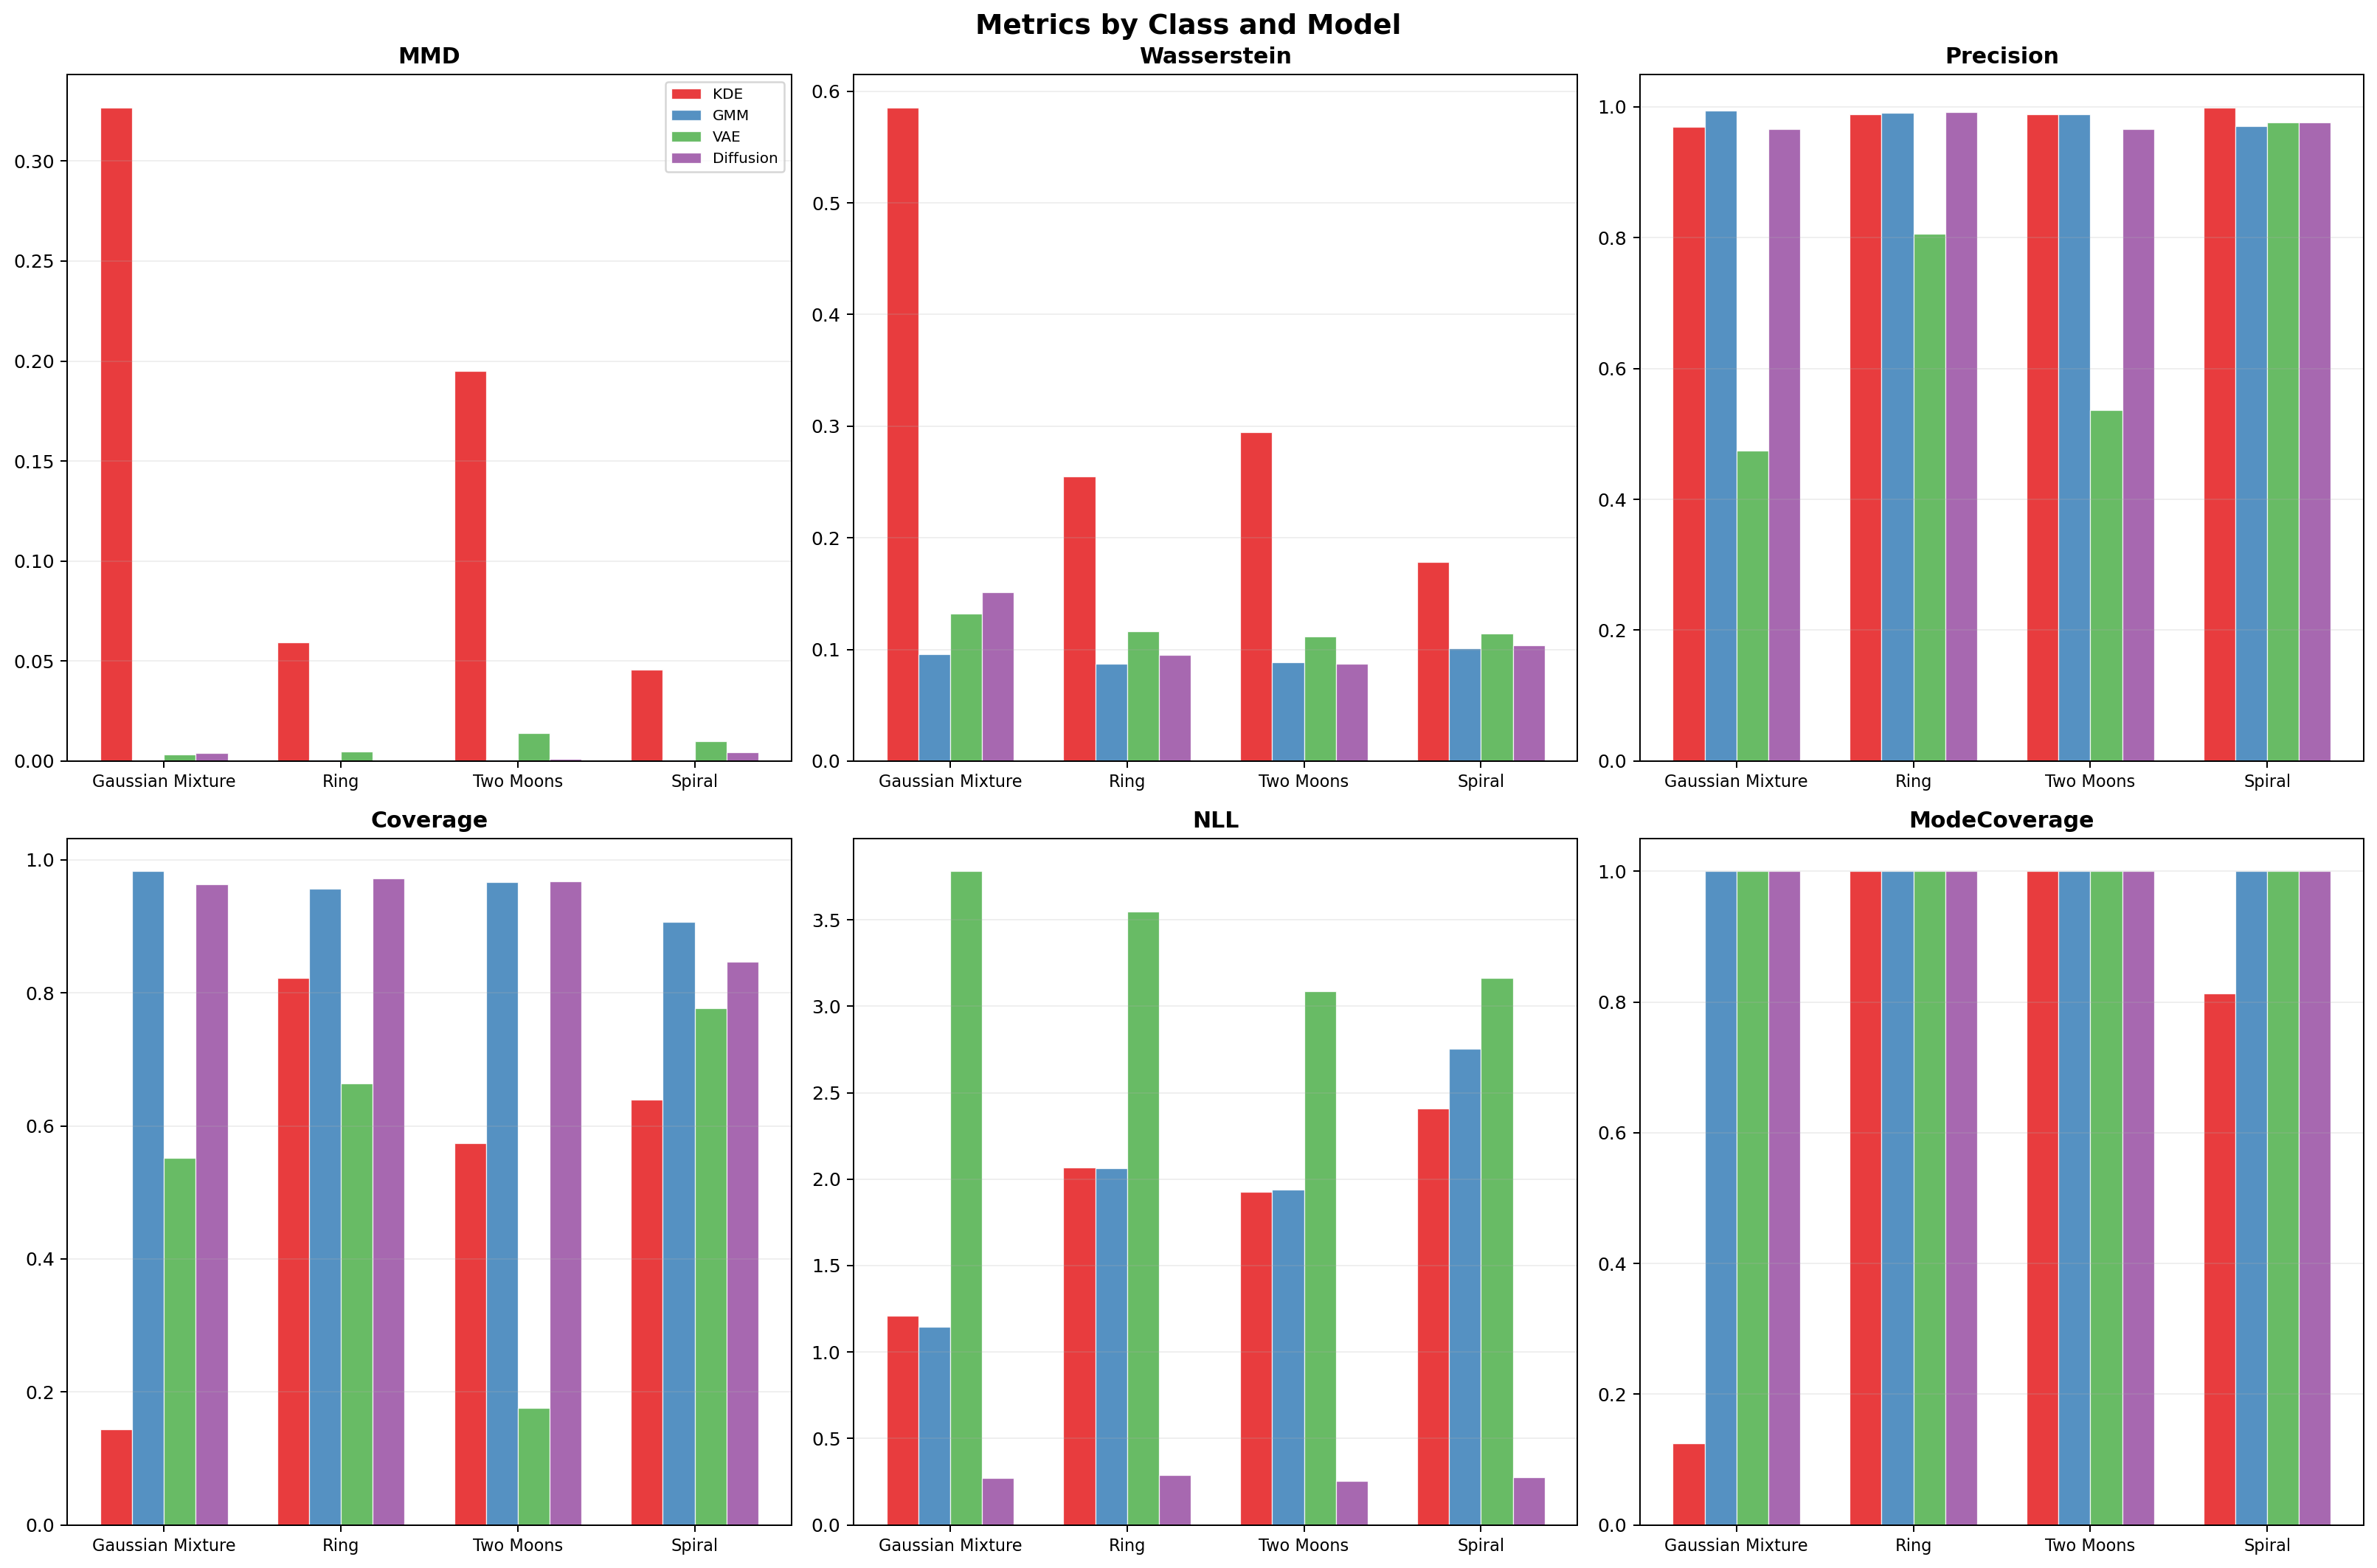
\includegraphics[width=0.92\textwidth]{metrics_bars.pdf}
    \caption{Coverage--Precision 平面与综合得分对比。左图中箭头表示从 VAE 到 DDPM 的质量变化方向，右图比较两类模型在不同分布上的综合得分。}
    \label{fig:metrics}
\end{figure}

表~\ref{tab:main_results} 和图~\ref{fig:metrics} 汇总了定量评价结果。表格给出各项指标的原始数值与最优模型，图~\ref{fig:metrics} 则突出 Coverage--Precision 平面中的质量变化方向和综合得分差异。在默认超参数和固定随机种子设置下，DDPM 在多数分布与多数指标上取得更优结果，尤其在 Ring 和 Two Moons 的支撑集保持上优势明显。不过，Gaussian Mixture 的全局分布指标中 VAE 仍有竞争力，Spiral 上两类模型也都未完全恢复精细的双臂结构。因此，主实验结果更适合作为后续失效机制分析的入口，而不是直接得出单一模型绝对占优的结论。

% ==================== 7. 结果分析与失效机制诊断 ====================
\section{结果分析与失效机制诊断}

\subsection{按分布分析：几何难度梯度的实验验证}

主实验结果与第三节给出的几何难度画像基本一致。Gaussian Mixture 的主要困难在于离散多峰覆盖，VAE 在 MMD 和 Wasserstein 等全局分布距离上仍有竞争力，但 Precision 偏低，说明其连续解码器会在团簇间低密度区域产生桥接样本。Ring 和 Two Moons 对支撑集形状更敏感，DDPM 在 Coverage 与 Precision 上优势明显，反映逐步去噪机制更容易保持薄流形和非凸分支。

Spiral 是最能区分模型失效机制的分布。DDPM 相比 VAE 更好地保持了宏观旋转趋势，但两类模型都没有稳定复现清晰的双臂中心线。这个现象说明 Spiral 不仅要求局部密度拟合，还要求全局相位顺序、螺旋臂身份和半径随相位变化关系保持一致。因此，Spiral 不能只作为一个普通测试集，而应作为诊断生成模型结构表达能力的压力测试。

\subsection{VAE 的潜空间诊断}

为解释 VAE 在 Two Moons 和 Spiral 上的生成失真，本文进一步检查编码后验、重构质量和先验采样质量。图~\ref{fig:vae_recon_prior} 对比了训练样本的重构结果与从标准高斯先验直接采样的生成结果。可以看到，VAE 对部分训练样本具有一定重构能力，但从先验采样时仍会出现桥接、增厚和云团化。这说明“能重构训练样本”并不等价于“能从先验稳定生成真实分布”。

\begin{figure}[!htbp]
    \centering
    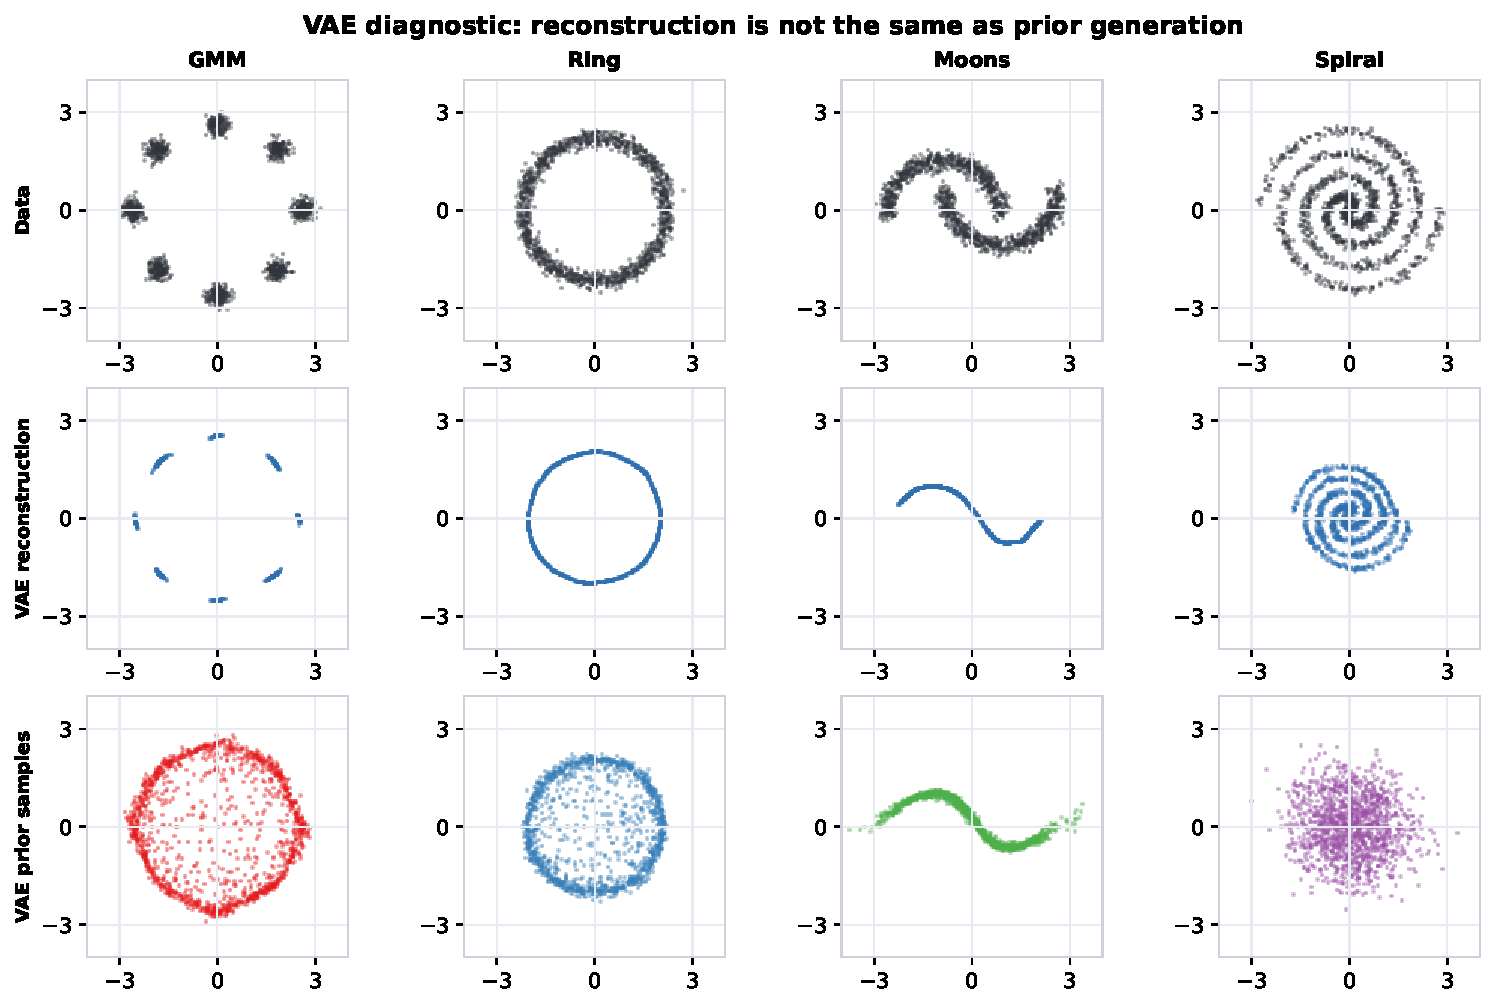
\includegraphics[width=0.92\textwidth]{vae_reconstruction_vs_prior.pdf}
    \caption{VAE 的重构样本与先验采样对比。重构结果说明编码器--解码器学习到部分局部图表；先验采样失真则表明标准高斯采样会穿过解码器未可靠学习的潜空间区域。}
    \label{fig:vae_recon_prior}
\end{figure}

逐维 KL 分析进一步揭示了失败原因。图~\ref{fig:vae_kl_dim} 显示，各类别的 KL 并未整体接近零，因此不能简单归结为典型的完全后验崩塌；但信息主要集中在少数潜变量维度中，每类通常只有 $1$--$2$ 个维度被有效使用。更准确的诊断是：VAE 出现了部分潜变量塌缩和潜空间低利用。

\begin{figure}[!htbp]
    \centering
    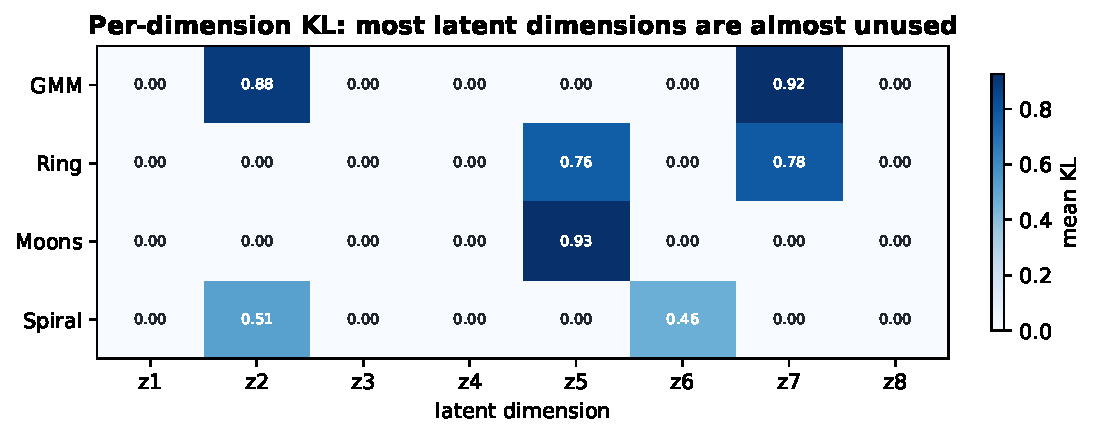
\includegraphics[width=0.82\textwidth]{vae_latent_kl_by_dim.pdf}
    \caption{VAE 逐维 KL 贡献。KL 未完全消失，但信息集中在少数潜变量维度中，说明模型并非完全后验崩塌，而是潜空间利用不足。}
    \label{fig:vae_kl_dim}
\end{figure}

从机制上看，ELBO 中的 KL 项将后验压向标准高斯先验，而重构项又要求模型表达多峰、闭合、分支和螺旋等复杂几何。二者折中后，潜空间形成低维而平滑的参数化。连续解码器在低密度潜空间区域进行插值，便会在数据支撑集之间生成不合理样本。这解释了 Gaussian Mixture 的团簇桥接、Ring 的环带增厚、Two Moons 的分支混合和 Spiral 的云团化。

\subsection{KL 弱化对 VAE 诊断的反向验证}

如果上述诊断成立，则适度减弱 KL 压缩应当改善 VAE 对复杂几何的覆盖。本文对 Two Moons 和 Spiral 进一步进行 $\beta$ sweep，比较
\[
    \beta\in\{1.0,0.3,0.1,0.03,0.01,0\}.
\]
结果如图~\ref{fig:vae_beta_sweep_metrics} 所示。Two Moons 在 $\beta=0.1$ 时达到较优 Coverage 和 MMD，Spiral 在 $\beta=0.3$ 附近表现最好。相较默认 $\beta=1.0$，适度弱化 KL 显著降低重构误差并提高覆盖能力，验证了 KL 压缩确实是 VAE 失真的重要来源。

图~\ref{fig:vae_beta_sweep_metrics} 中除通用生成指标外，还包含三个用于解释 VAE 机制的诊断量。其一，\textbf{Off-support} 表示离支撑比例：以测试集样本的第 5 近邻半径的 $95\%$ 分位数作为真实支撑集厚度阈值，若生成样本到最近测试样本的距离超过该阈值，则记为离开真实支撑集；该值越小说明生成样本越少落在月牙间隙、螺旋臂外侧等低密度区域。其二，\textbf{Recon MSE} 是训练样本经编码器取后验均值再解码后的平均重构误差 $\mathbb{E}\norm{\hat{\vect{x}}-\vect{x}}^2$，衡量模型对已见数据局部结构的重构能力。其三，\textbf{KL} 是 VAE 损失中的平均 KL 正则项
\[
    \frac{1}{2}\sum_{j=1}^{d}\left(\mu_j^2+\sigma_j^2-\log\sigma_j^2-1\right),
\]
衡量编码后验偏离标准高斯先验的程度。Recon MSE 越小通常表示重构越好，KL 越小表示潜空间越规整；但若 KL 过小会压缩几何信息，若 KL 过大则说明编码区域与标准高斯先验脱节，都会影响从先验采样的生成质量。

\begin{figure}[!htbp]
    \centering
    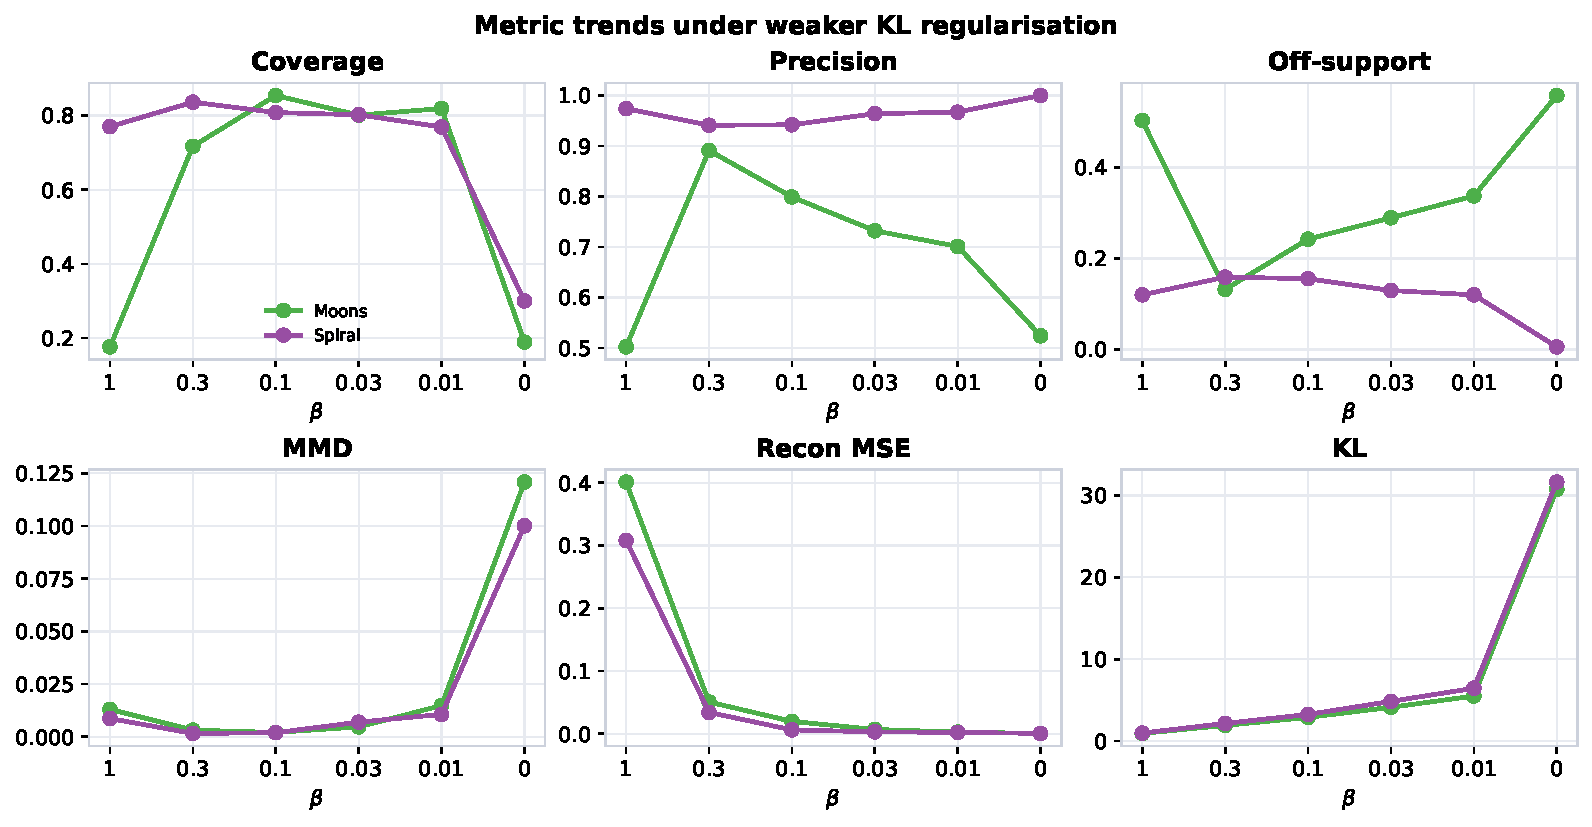
\includegraphics[width=0.90\textwidth]{vae_beta_sweep_metrics.pdf}
    \caption{VAE 的 KL 权重敏感性实验。Off-support、Recon MSE 和 KL 分别刻画离支撑比例、重构误差和潜空间正则强度；适度降低 $\beta$ 能改善 Two Moons 和 Spiral 的覆盖，但过弱 KL 会破坏先验采样可靠性。}
    \label{fig:vae_beta_sweep_metrics}
\end{figure}

图~\ref{fig:vae_beta_sweep_samples} 给出了对应的先验采样结果。相比单纯查看指标，样本图更直观地显示：适度降低 $\beta$ 后，Two Moons 的两条弧形分支更连续，Spiral 的云团化有所缓解；但当 $\beta$ 过小时，生成样本开始变得过散或偏离真实支撑集。

\begin{figure}[!htbp]
    \centering
    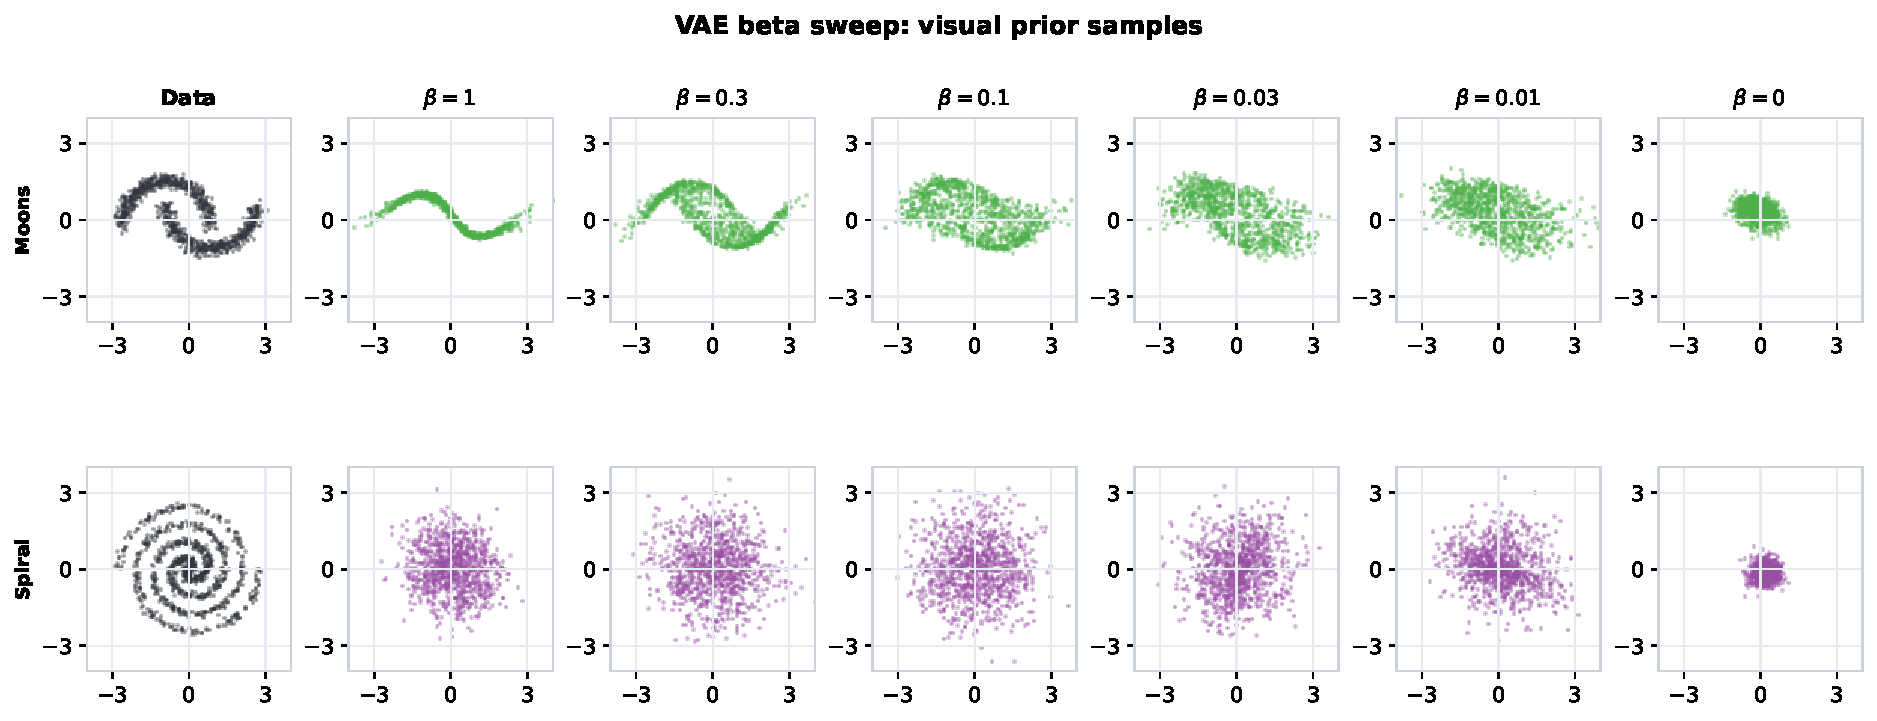
\includegraphics[width=0.96\textwidth]{vae_beta_sweep_samples.pdf}
    \caption{不同 KL 权重下 VAE 从标准高斯先验采样的直观结果。适度弱化 KL 可改善覆盖，但过弱 KL 会削弱潜空间规整性，使先验采样落入解码器未可靠学习的区域。}
    \label{fig:vae_beta_sweep_samples}
\end{figure}

因此，$\beta$ 并非越小越好。当 $\beta$ 降至 $0.03$、$0.01$ 甚至 $0$ 时，重构误差继续下降，但无条件先验采样反而恶化。特别是 $\beta=0$ 时，模型接近普通自编码器：训练样本可以被准确重构，但编码区域与标准高斯先验严重脱节，从 $z\sim\mathcal{N}(0,I)$ 采样不再可靠。由此可见，VAE 的关键矛盾不是单纯容量不足，而是“几何表达能力”和“先验可采样性”之间的结构性权衡。

\subsection{DDPM 的优势来源与 Spiral 局限}

DDPM 的优势主要来自逐步去噪机制。与 VAE 从单一高斯潜空间一次性解码不同，DDPM 将生成过程拆成多个噪声水平下的局部去噪任务，因而较少出现由潜空间插值导致的桥接和填充。这解释了 DDPM 在 Ring 与 Two Moons 上更好的支撑集保持能力。

但 Spiral 的补充实验表明，DDPM 的局部去噪优势并不自动保证全局拓扑一致性。本文比较了原始 DDPM、较短线性扩散链、cosine 噪声调度和加入极坐标特征的 DDPM。图~\ref{fig:diffusion_spiral_samples} 显示，轻量调度或极坐标特征只能有限改变点云形状，仍难以稳定恢复清晰双臂中心线。

\begin{figure}[!htbp]
    \centering
    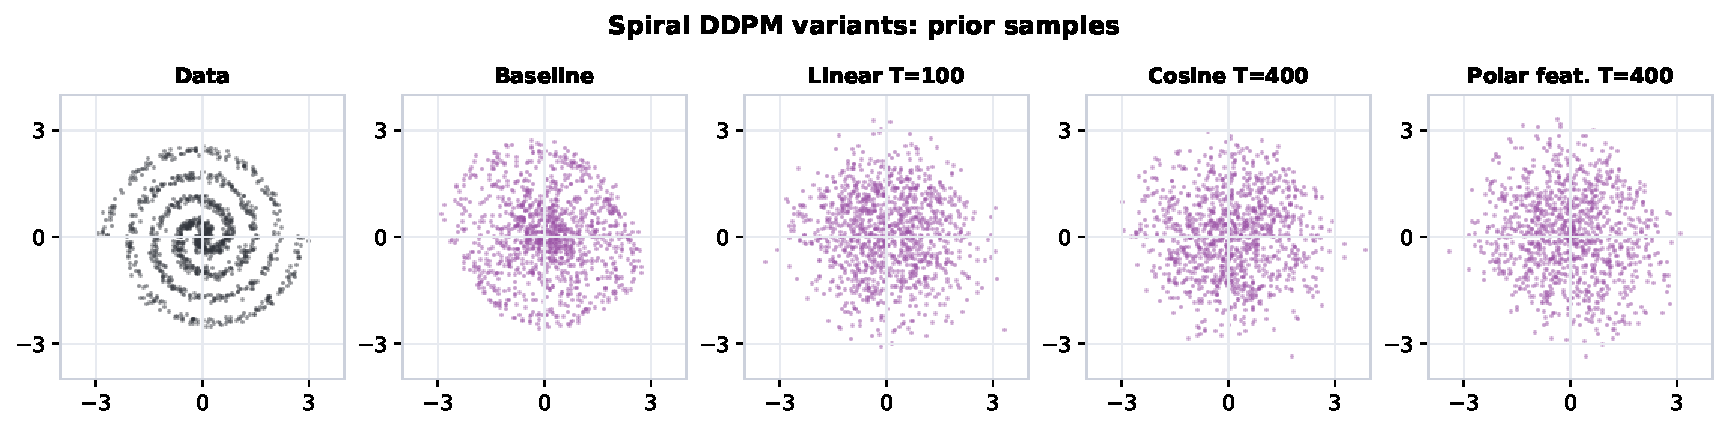
\includegraphics[width=0.94\textwidth]{diffusion_spiral_samples.pdf}
    \caption{Spiral 上的 DDPM 调整实验。减少步数、使用 cosine 调度或加入极坐标特征均不能从根本上恢复清晰双臂螺旋。}
    \label{fig:diffusion_spiral_samples}
\end{figure}

因此，DDPM 相比 VAE 的优势在于避免单步潜空间解码和低密度插值，但 Spiral 暴露出另一层困难：普通 DDPM 学到的是局部 score 场，而双臂螺旋要求模型同时维护相位顺序、螺旋臂身份和半径--相位关系。这为下一节引入结构先验提供了直接动机。

\subsection{质量、效率与结构表达的权衡}

综合来看，VAE 的优势是训练稳定、采样极快和目标函数清晰；其短板是标准高斯先验与复杂非欧几何之间存在张力。DDPM 的优势是局部几何保持和支撑集覆盖；其短板是采样成本较高，且在 Spiral 这类长程相位结构上缺少显式约束。两类模型并非简单强弱关系，而是在生成效率、局部精度、先验可采样性和结构表达能力之间采取了不同折中。

% ==================== 8. 拓展实验与结构增强 ====================
\section{拓展实验与结构增强}

\subsection{超参数敏感性：VAE 的 KL 权重与 DDPM 的扩散配置}

第七节的诊断说明，VAE 的关键超参数是 KL 权重 $\beta$，DDPM 的关键问题则不完全在扩散步数。图~\ref{fig:vae_beta_sweep_metrics} 已经表明，VAE 在 $\beta=0.3$--$0.1$ 区间明显优于默认配置，但继续弱化 KL 会损害先验采样。DDPM 在 Spiral 上的变体实验进一步表明，减少步数、改变噪声调度或加入极坐标特征都不能完全解决双臂相位结构问题。

这组超参数结果修正了主实验中的简单排序：默认配置下 DDPM 更稳，但 VAE 经过适度 KL 调整后可以显著改善复杂流形覆盖；同时，DDPM 的瓶颈不只是采样步数，而是普通坐标与局部去噪目标对全局结构的表达不足。

\subsection{螺旋结构先验增强}

基于前述诊断，本文进一步提出 Spiral 的结构先验增强实验。核心思想是将二维坐标生成问题拆解为更符合数据机理的变量：
\[
    \text{sample} = \text{arm label} + \text{phase } t + \text{local residual}.
\]
具体地，用双臂阿基米德螺旋中心线描述主结构：
\begin{equation}
    \vect{c}_a(t)=\alpha t
    \begin{bmatrix}
    \cos(t+a\pi)\\
    \sin(t+a\pi)
    \end{bmatrix},
    \qquad a\in\{0,1\}.
\end{equation}
从训练数据拟合得到 $\alpha=0.2200$，相位范围约为 $[0.160,12.568]$，法向残差标准差约为 $0.0779$。每个样本被投影到最近的螺旋臂和相位位置，从而得到臂编号、相位和法向残差。

本文比较两类增强：第一，\textbf{Spiral-coordinate DDPM} 在归一化相位和法向残差坐标中训练 DDPM，采样后再映射回二维平面；第二，\textbf{Spiral structural prior} 直接从拟合的臂编号、相位范围和经验残差分布中采样。后者不是与 VAE/DDPM 完全公平竞争的黑盒模型，而是用于验证显式结构先验是否能恢复 Spiral 几何的诊断性上界。

由于本节关注的是双臂中心线和全局相位结构，单独使用 Wasserstein 距离并不足以区分“整体点云位置接近”和“严格沿螺旋轨迹生成”。例如，生成样本如果落在真实点云包络附近但填充了两条螺旋臂之间的空白区域，Wasserstein 距离可能仍然不高，但这种结果在结构上是失败的。因此，结构增强实验保留 MMD、Coverage 和 Precision 作为与主实验对齐的通用指标，同时引入两个 Spiral 专用结构指标。

\textbf{结构指标说明。} 记拟合得到的双臂螺旋中心线集合为
\[
    \mathcal{C}=\{\vect{c}_a(t):a\in\{0,1\},\ t\in[t_{\min},t_{\max}]\},
    \qquad
    d_{\mathcal{C}}(\vect{x})=\min_{\vect{c}\in\mathcal{C}}\norm{\vect{x}-\vect{c}}_2 .
\]
令 $\tau$ 为真实样本到中心线距离 $\{d_{\mathcal{C}}(\vect{x}_i)\}$ 的 $95\%$ 分位数，则\textbf{曲线外比例}定义为
\[
    \mathrm{CurveOff}(Y)
    =\frac{1}{|Y|}\sum_{\vect{y}\in Y}\mathbf{1}
    \{d_{\mathcal{C}}(\vect{y})>\tau\}.
\]
该指标越小，说明生成样本越贴近双臂螺旋支撑集。另一方面，将样本投影到最近的“臂编号--相位”坐标后，可得到真实样本和生成样本的二维直方图 $\hat p_{\mathrm{real}}(a,t)$ 与 $\hat p_{\mathrm{gen}}(a,t)$。本文将二者的 Jensen--Shannon 散度记为\textbf{相位 JS 散度}：
\[
    \mathrm{PhaseJS}
    =\operatorname{JS}\!\left(\hat p_{\mathrm{real}}(a,t),\hat p_{\mathrm{gen}}(a,t)\right).
\]
Phase JS 越小，说明生成样本越能覆盖完整螺旋相位，并在两条螺旋臂上的分布越接近真实数据。简言之，CurveOff 判断“是否贴在曲线上”，Phase JS 判断“是否沿曲线按正确相位展开”。

\begin{figure}[!htbp]
    \centering
    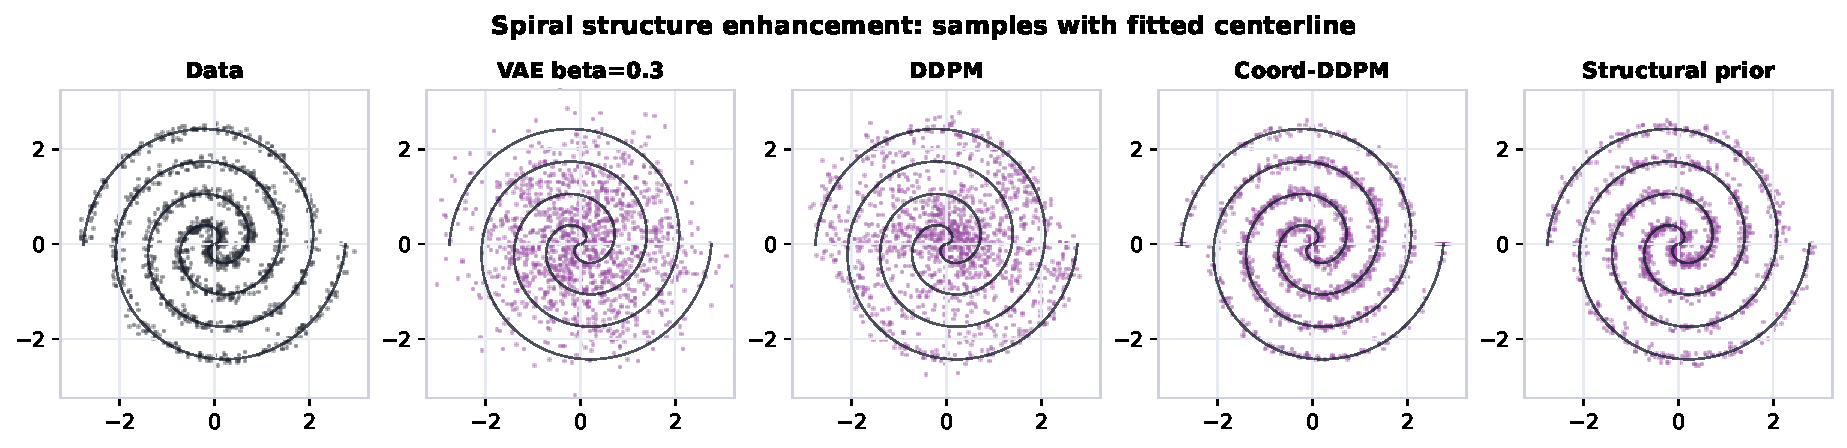
\includegraphics[width=0.96\textwidth]{spiral_structure_samples.pdf}
    \caption{螺旋结构先验增强的样本对比。VAE 和普通 DDPM 均有云团化与离中心线现象；结构坐标 DDPM 和结构先验生成器基本沿双臂中心线生成样本。}
    \label{fig:spiral_structure_samples}
\end{figure}

\begin{table}[!htbp]
\centering
\small
\caption{Spiral 结构增强实验结果}
\label{tab:spiral_structure}
\begin{tabular}{lcccc}
\toprule
方法 & MMD$\downarrow$ & Cov.$\uparrow$ & Prec.$\uparrow$ & 曲线外比例$\downarrow$ \\
\midrule
VAE $\beta=0.3$ & 0.0011 & 0.841 & 0.919 & 0.535 \\
DDPM baseline & 0.0025 & 0.839 & 0.938 & 0.487 \\
Spiral-coordinate DDPM & \textbf{0.0004} & 0.949 & \textbf{1.000} & \textbf{0.048} \\
Spiral structural prior & 0.0014 & \textbf{0.957} & 0.999 & 0.051 \\
\bottomrule
\end{tabular}
\end{table}

表~\ref{tab:spiral_structure} 和图~\ref{fig:spiral_structure_samples} 给出了最直接的验证结果。普通 DDPM 的曲线外比例为 $0.487$，说明大量样本虽然位于 Spiral 数据云附近，但没有严格沿双臂中心线分布；Spiral-coordinate DDPM 将该比例降至 $0.048$，同时 MMD 降至 $0.0004$，Coverage 提升至 $0.949$。图~\ref{fig:spiral_structure_metrics} 进一步展示了曲线外比例、相位 JS、Coverage 和 MMD 的对比，其中相位 JS 用于补充判断样本是否沿螺旋相位均匀展开。这说明 Spiral 的主要瓶颈不是网络容量或扩散步数，而是原始坐标下缺少显式相位和分支约束。

\begin{figure}[!htbp]
    \centering
    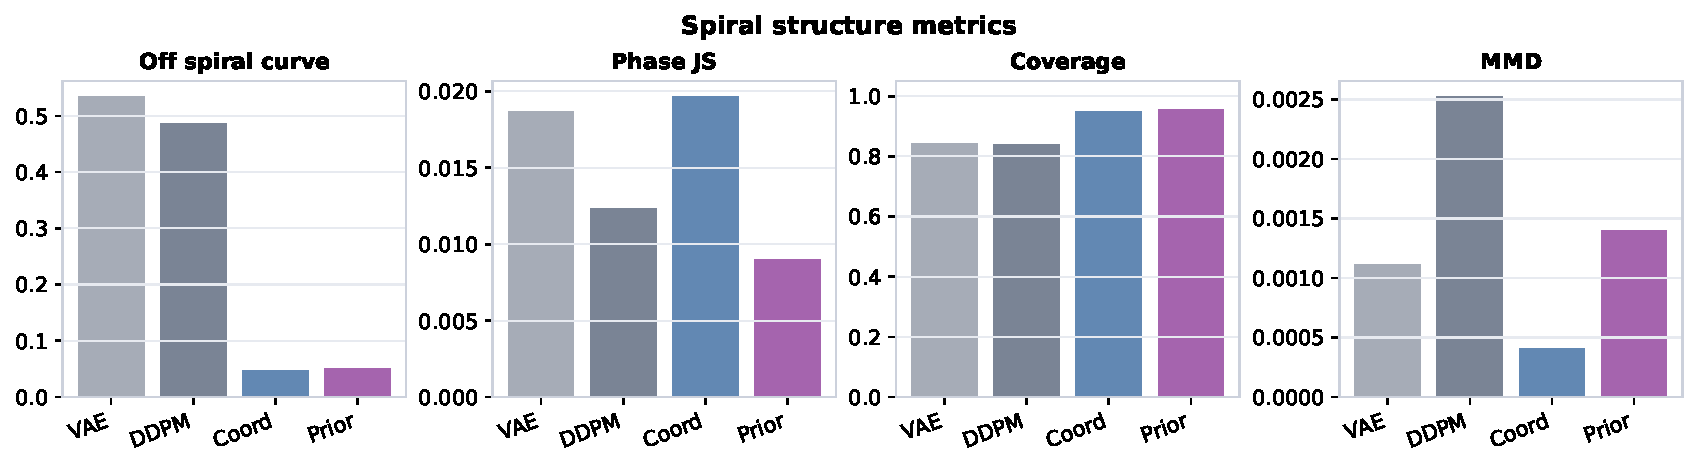
\includegraphics[width=0.92\textwidth]{spiral_structure_metrics.pdf}
    \caption{Spiral 结构增强的指标对比。曲线外比例衡量样本偏离螺旋中心线的程度，Phase JS 衡量投影到螺旋相位后的分布一致性；结构坐标 DDPM 和结构先验方法显著降低曲线外比例，并提高 Coverage。}
    \label{fig:spiral_structure_metrics}
\end{figure}

这一结果把全文主线闭合起来：VAE 失败主要来自 KL 压缩和连续解码插值；DDPM 规避了这一问题，因此整体更稳；但对于 Spiral，普通 DDPM 仍缺少全局相位结构。将生成空间改写为“螺旋臂--相位--局部残差”后，模型能够更直接地恢复双臂螺旋。这说明复杂生成任务不仅需要更强网络，还需要与数据机理相匹配的结构化表示。

\subsection{条件生成}

主实验中每类分布独立训练模型。为覆盖统一可控生成任务，本文在四类联合数据集上训练条件 VAE 和条件 DDPM，将 one-hot 类别标签作为额外条件输入。条件模型学习
\[
    p_{\theta}(\vect{x}\mid c),\qquad c\in\{1,2,3,4\},
\]
使同一组参数能够根据类别标签生成不同分布。

\begin{table}[!htbp]
\centering
\small
\caption{条件生成模型在四类分布上的性能}
\label{tab:conditional_new}
\begin{tabular}{llccccc}
\toprule
分布 & 模型 & MMD$\downarrow$ & Wass.$\downarrow$ & Cov.$\uparrow$ & Prec.$\uparrow$ & 综合得分$\uparrow$ \\
\midrule
\multirow{2}{*}{Gaussian Mixture} & CVAE & 0.0619 & 0.120 & 0.666 & 0.494 & 0.296 \\
                                  & 条件DDPM & \textbf{0.0431} & \textbf{0.110} & \textbf{0.958} & \textbf{0.978} & \textbf{0.765} \\
\midrule
\multirow{2}{*}{Ring} & CVAE & 0.0603 & 0.106 & 0.668 & 0.852 & 0.583 \\
                      & 条件DDPM & \textbf{0.0295} & \textbf{0.086} & \textbf{0.928} & \textbf{0.996} & \textbf{0.988} \\
\midrule
\multirow{2}{*}{Two Moons} & CVAE & 0.1035 & 0.118 & 0.186 & 0.630 & 0.079 \\
                           & 条件DDPM & \textbf{0.0296} & \textbf{0.094} & \textbf{0.956} & \textbf{0.990} & \textbf{0.935} \\
\midrule
\multirow{2}{*}{Spiral} & CVAE & 0.0956 & 0.117 & 0.788 & \textbf{1.000} & 0.491 \\
                        & 条件DDPM & \textbf{0.0718} & \textbf{0.111} & \textbf{0.882} & 0.994 & \textbf{0.647} \\
\bottomrule
\end{tabular}
\end{table}

\begin{figure}[!htbp]
    \centering
    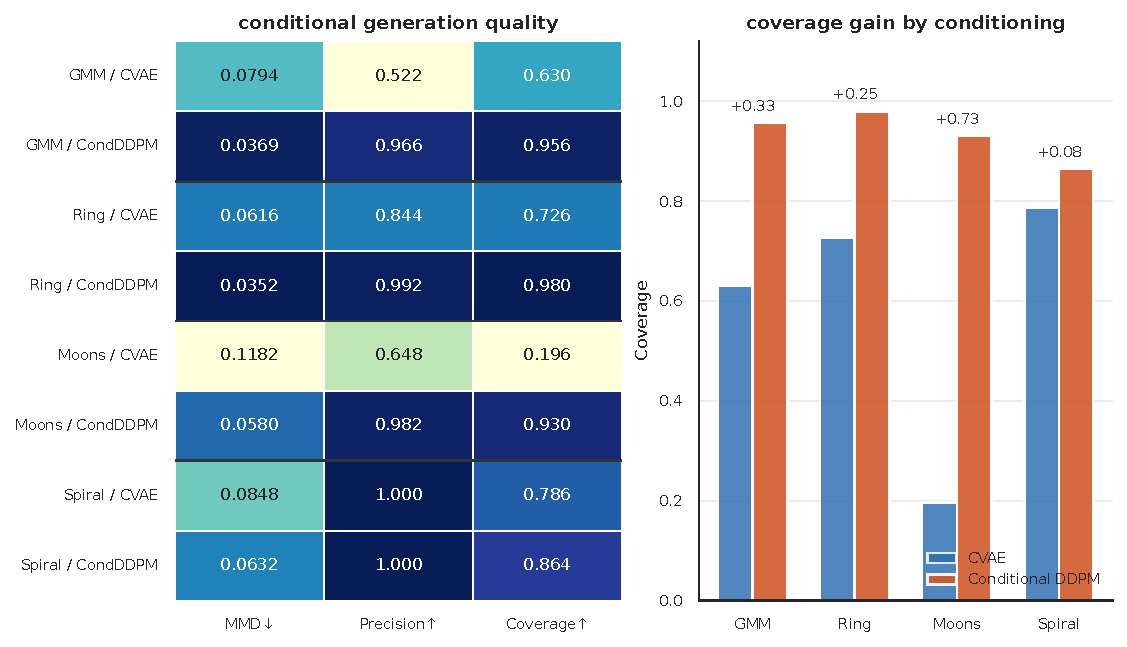
\includegraphics[width=0.92\textwidth]{conditional_metrics.pdf}
    \caption{条件生成模型的 Coverage--Precision 平面与综合得分对比。左图中箭头表示从 CVAE 到条件 DDPM 的质量变化方向，右图比较两类条件模型在不同分布上的综合得分。}
    \label{fig:conditional_new}
\end{figure}

表~\ref{tab:conditional_new} 与主实验表格保持一致，给出四项原始指标和综合得分；图~\ref{fig:conditional_new} 则采用相同的 Coverage--Precision 平面和综合得分柱状对比。综合得分由 MMD、Wasserstein、Coverage 和 Precision 归一化后等权平均得到。结果显示，条件 DDPM 在多数指标上优于 CVAE，说明主实验中的范式差异在统一条件生成场景下仍然存在。最明显的差异来自 Coverage：条件 DDPM 在四类分布上均保持 $0.882$ 以上，而 CVAE 在 Two Moons 上仅为 $0.186$。这表明类别标签本身并不能消除 VAE 的潜空间插值问题；当目标分布具有明显非凸分支时，CVAE 仍会受到标准高斯先验和连续解码器的共同限制。条件 DDPM 则通过类别条件约束去噪方向，在统一模型中保持了较稳定的类内支撑集覆盖。

\subsection{异常点鲁棒性分析}

为评估数据受污染时的稳定性，本文在 Spiral 训练集中混入比例为 $\rho\in\{0\%,5\%,10\%\}$ 的污染样本，并重新训练 VAE 与 DDPM。为避免鲁棒性结论只依赖单一噪声形态，本文设置三类污染机制：
\[
\begin{aligned}
\text{均匀异常点：}\quad & \vect{x}_{\mathrm{out}}\sim U([-4,4]^2),\\
\text{团簇偏移：}\quad & \vect{x}_{\mathrm{out}}=\vect{x}_i+(1.20,-1.00)+\vect{\epsilon},\quad \vect{\epsilon}\sim \Ncal(0,0.06^2\vect{I}),\\
\text{异方差噪声：}\quad & \vect{x}_{\mathrm{out}}=\vect{x}_i+\sigma(r_i)\epsilon_r\vect{u}_r+0.35\sigma(r_i)\epsilon_t\vect{u}_t .
\end{aligned}
\]
三者分别对应无结构离群点、结构化伪模式和局部流形厚度扰动。表~\ref{tab:robust_new} 汇总 $10\%$ 污染下的完整指标，图~\ref{fig:robust_new} 展示三类污染随比例增加的退化趋势。

\begin{table}[!htbp]
\centering
\small
\caption{$10\%$ 污染下三类污染机制的鲁棒性实验（Spiral）}
\label{tab:robust_new}
\begin{tabular}{llccccc}
\toprule
污染机制 & 模型 & MMD$\downarrow$ & Wass.$\downarrow$ & Cov.$\uparrow$ & Prec.$\uparrow$ & 综合得分$\uparrow$ \\
\midrule
\multirow{2}{*}{均匀异常点} & VAE  & \textbf{0.0431} & \textbf{0.106} & 0.884 & \textbf{0.960} & \textbf{0.786} \\
                            & DDPM & 0.0923 & 0.110 & \textbf{0.914} & 0.902 & 0.506 \\
\midrule
\multirow{2}{*}{团簇偏移} & VAE  & \textbf{0.0907} & \textbf{0.114} & 0.814 & \textbf{0.988} & \textbf{0.421} \\
                          & DDPM & 0.1180 & 0.122 & \textbf{0.886} & 0.954 & 0.313 \\
\midrule
\multirow{2}{*}{异方差噪声} & VAE  & 0.0953 & 0.119 & 0.834 & \textbf{1.000} & 0.413 \\
                            & DDPM & \textbf{0.0613} & \textbf{0.104} & \textbf{0.860} & \textbf{1.000} & \textbf{0.804} \\
\bottomrule
\end{tabular}
\end{table}

\begin{figure}[!htbp]
    \centering
    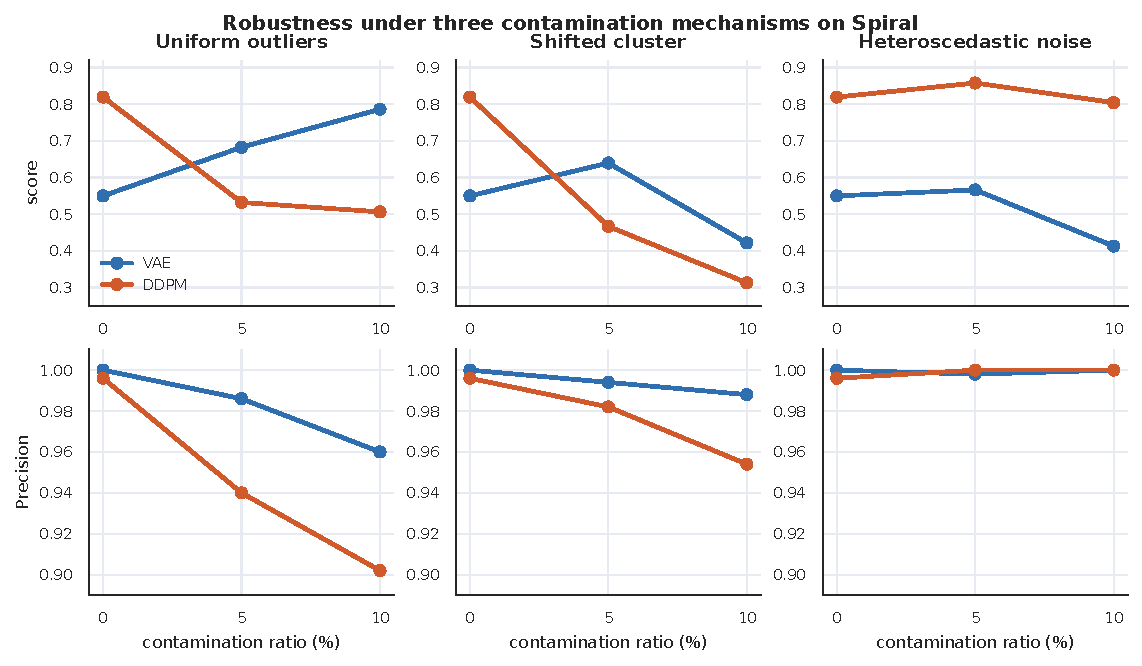
\includegraphics[width=0.92\textwidth]{robustness_curves.pdf}
    \caption{Spiral 分布在三类污染机制下的鲁棒性曲线。上排为基于 MMD、Wasserstein、Coverage 和 Precision 归一化得到的综合得分，下排为 Precision；横轴为污染比例。}
    \label{fig:robust_new}
\end{figure}

表~\ref{tab:robust_new} 和图~\ref{fig:robust_new} 表明，污染类型会显著改变模型排序。在均匀异常点下，VAE 的 Precision 保持更好，$10\%$ 污染时综合得分为 $0.786$，高于 DDPM 的 $0.506$；这说明 KL 正则和连续潜空间对无结构离群点有一定平滑作用。团簇偏移是更困难的设置，因为污染点本身形成局部伪模式。两类模型在该设置下均退化，其中 DDPM 的 MMD 和 Wasserstein 上升更明显，反映结构化污染会直接干扰 score 估计。异方差噪声下则相反，DDPM 在 $10\%$ 污染时综合得分达到 $0.804$，明显高于 VAE 的 $0.413$，说明逐步去噪机制更适合吸收沿流形厚度变化的局部扰动。

因此，鲁棒性不能简单概括为某一类模型绝对更强。VAE 对无结构异常点更稳，但面对局部厚度变化时容易过平滑；DDPM 在干净数据和异方差扰动下保持较好几何质量，但对结构化伪模式更敏感。这个结论与前文失效机制一致：VAE 的正则化带来过滤噪声的能力，也限制了细几何表达；DDPM 的局部 score 学习能刻画流形厚度，却会认真学习训练集中持续存在的结构化污染。

% ==================== 9. 结论与展望 ====================
\section{结论与展望}

\subsection{主要结论}

本文以 Gaussian Mixture、Ring、Two Moons 和 Spiral 四类二维分布为平台，比较 VAE 与 DDPM 的生成能力，并通过诊断实验进一步解释两类模型的失效机制。主要结论如下：

\begin{enumerate}[label=(\arabic*)]
    \item 四类数据形成了从离散多峰到复杂拓扑流形的难度梯度。二维可视化和局部几何统计能够有效揭示不同分布的建模难点。
    \item 在默认配置下，DDPM 在多数几何分布上优于 VAE，尤其在局部支撑保持和流形覆盖方面更稳；但 Gaussian Mixture 的全局指标中 VAE 仍有竞争力，说明二者并非简单强弱关系。
    \item VAE 的失败不是典型完全后验崩塌，而是部分潜变量塌缩、潜空间低利用和连续解码插值共同造成。适度弱化 KL 能改善覆盖，但过弱 KL 会破坏标准高斯先验采样。
    \item DDPM 规避了 VAE 的单步潜空间解码问题，因此更少产生桥接和填充；但普通 DDPM 在 Spiral 上仍缺少全局相位和分支结构约束。
    \item 螺旋结构先验增强显著改善 Spiral。结构坐标 DDPM 将曲线外比例从普通 DDPM 的 $0.487$ 降至 $0.048$；该实验不是为了构造通用黑盒模型的公平替代，而是作为诊断性验证，说明“结构变量显式化”对复杂拓扑生成具有关键作用。
    \item 条件生成和鲁棒性实验补充说明了两类模型的适用边界：条件 DDPM 在统一可控生成中保持优势；鲁棒性则依赖污染机制，VAE 对无结构异常点更稳，DDPM 对异方差流形扰动更稳。
\end{enumerate}

\subsection{不足与展望}

本文仍有三点局限。第一，实验数据为二维分布，便于解释和可视化，但向高维真实数据外推需要谨慎。第二，部分结论基于固定随机种子和当前网络配置，若进行多随机种子统计，结论应进一步以均值和标准差表述。第三，螺旋结构增强利用了较强的几何先验，它证明了结构化建模的价值，但不应被解释为通用黑盒生成器的公平替代。

未来工作可以从三个方向展开：其一，引入 Normalizing Flow 或可逆坐标变换模型，系统比较结构化坐标建模与扩散模型的关系；其二，将“相位--分支--局部残差”的思想推广到更复杂的曲线、曲面或科学仿真数据；其三，探索 DDIM 等快速采样方法，在保持 DDPM 几何质量的同时降低采样成本。

% ==================== 参考文献 ====================
\begin{thebibliography}{99}

\bibitem{kingma2014vae}
Kingma, D. P. and Welling, M.
\newblock Auto-encoding variational Bayes.
\newblock \emph{International Conference on Learning Representations (ICLR)}, 2014.

\bibitem{ho2020ddpm}
Ho, J., Jain, A., and Abbeel, P.
\newblock Denoising diffusion probabilistic models.
\newblock \emph{Advances in Neural Information Processing Systems (NeurIPS)}, 33:6840--6851, 2020.

\bibitem{gretton2012mmd}
Gretton, A., Borgwardt, K. M., Rasch, M. J., Sch\"{o}lkopf, B., and Smola, A.
\newblock A kernel two-sample test.
\newblock \emph{Journal of Machine Learning Research}, 13(25):723--773, 2012.

\bibitem{rabin2011swd}
Rabin, J., Peyr\'{e}, G., Delon, J., and Bernot, M.
\newblock Wasserstein barycenter and its application to texture mixing.
\newblock In \emph{Scale Space and Variational Methods in Computer Vision (SSVM)}, pages 435--446, 2011.

\bibitem{kyukaaniemi2019prdc}
Kynk\"{a}\"{a}nniemi, T., Karras, T., Laine, S., Lehtinen, J., and Aila, T.
\newblock Improved precision and recall metric for assessing generative models.
\newblock \emph{Advances in Neural Information Processing Systems (NeurIPS)}, 32, 2019.

\end{thebibliography}

% ==================== 附录 ====================
\appendix
\section{补充可视化}

正文图~\ref{fig:gen} 采用 KDE 等高线压缩展示主实验生成效果。为便于直接观察样本级差异，附录图~\ref{fig:appendix_main_samples} 给出四类分布上真实数据、VAE 生成样本和 DDPM 生成样本的完整散点对比。

\begin{figure}[!htbp]
    \centering
    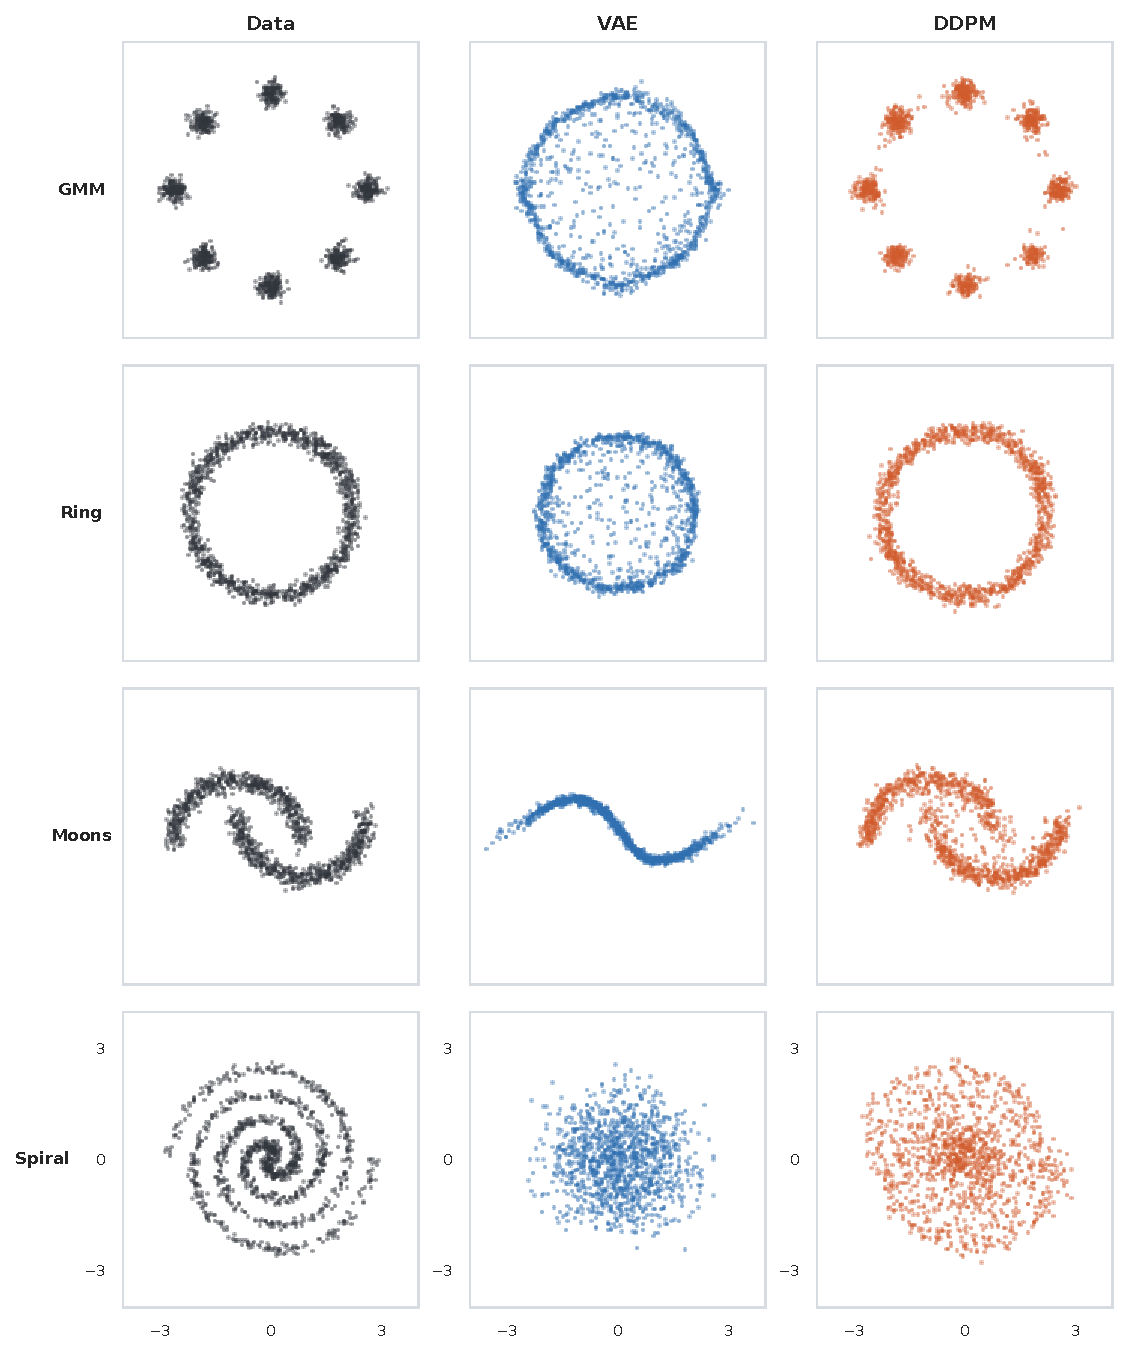
\includegraphics[width=0.92\textwidth]{main_generation_grid.pdf}
    \caption{主实验完整样本对比。每行对应一个分布，每列分别为真实数据、VAE 生成样本和 DDPM 生成样本。}
    \label{fig:appendix_main_samples}
\end{figure}

在诊断和拓展实验之后，本文还可以为每类分布选择当前实验链条中的最优生成方案。Gaussian Mixture、Ring 和 Two Moons 采用主实验中整体表现更稳的 DDPM；Spiral 则采用第八节提出的螺旋坐标 DDPM，以显式相位和臂结构约束弥补普通 DDPM 的全局拓扑不足。附录图~\ref{fig:appendix_best_samples} 给出这些优化后生成样本与真实数据的直接对照。

\begin{figure}[!htbp]
    \centering
    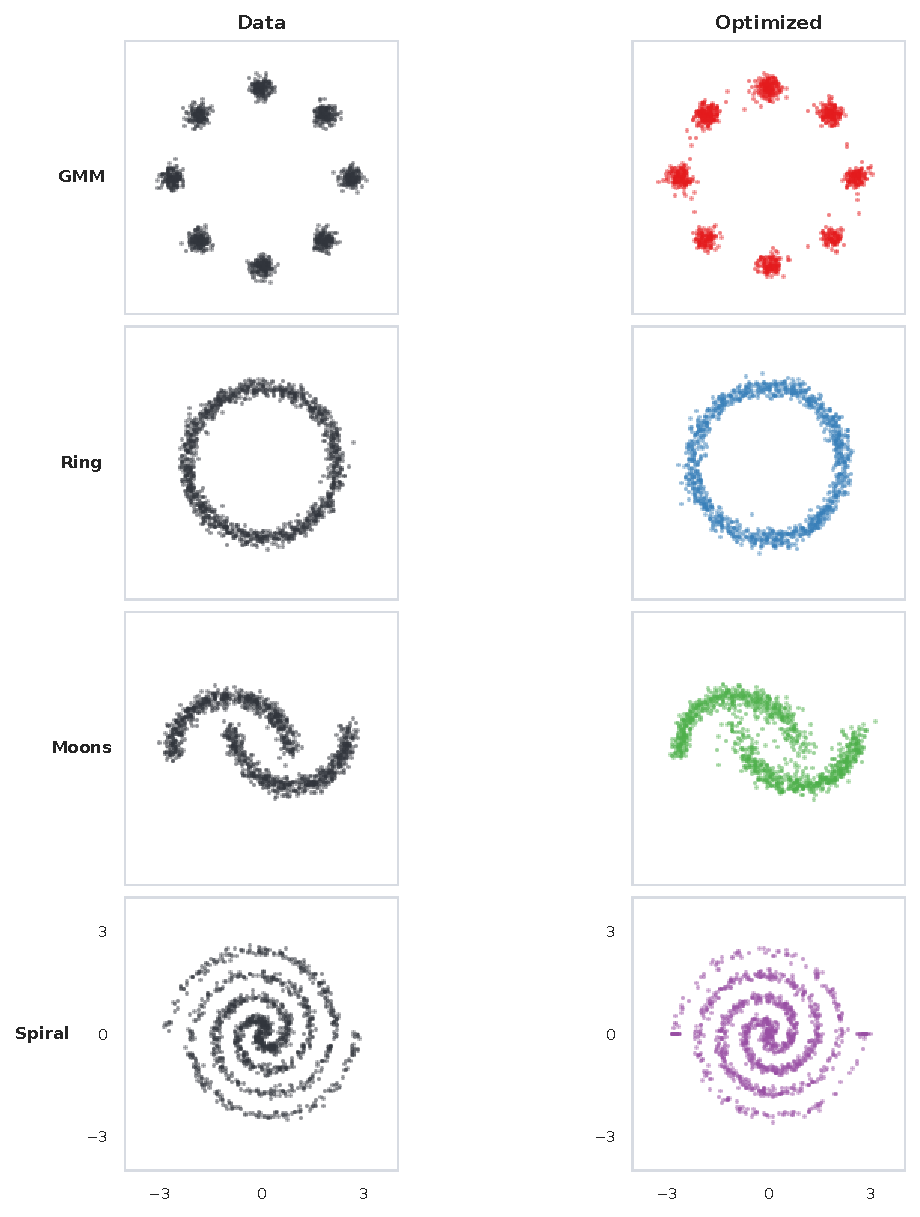
\includegraphics[width=0.88\textwidth]{optimized_generation_grid.pdf}
    \caption{拓展实验后的优化生成效果。前三类分布采用 DDPM，Spiral 采用 Spiral-coordinate DDPM；该图展示了本文经过诊断和结构增强后可达到的最佳样本级效果。}
    \label{fig:appendix_best_samples}
\end{figure}

\end{document}
